\documentclass[10pt,a4paper]{article}
\usepackage[utf8]{inputenc}
\usepackage[T1]{fontenc}
\usepackage{lmodern}
\usepackage[margin=1.75cm]{geometry}
\usepackage{amsmath,amssymb,amsfonts}
\usepackage{booktabs}
\usepackage{graphicx}
\usepackage{float}
\usepackage[section]{placeins}
\usepackage{hyperref}
\usepackage{xcolor}
\usepackage{caption}

\hypersetup{
    colorlinks=true,
    linkcolor=blue!60!black,
    citecolor=blue!60!black,
    urlcolor=blue!60!black
}

\title{Safe and Smooth Automatic Train Speed Control:\\
From State-Augmented MPC to Multi-Station Hierarchical\\
Differential and Assume-Guarantee Contract Shielding}
\author{Technical Report}
\date{\today}

\begin{document}
\maketitle

\begin{abstract}
Modern railway automation splits longitudinal train control into two disconnected layers: Automatic Train Protection (ATP), which guarantees safety through conservative worst-case braking envelopes and rigid speed ceilings, and Automatic Train Operation (ATO), which seeks comfortable acceleration profiles, low traction energy, punctual station arrivals, and accurate platform docking without formal multi-property guarantees. Our objective is to merge ATP safety certification and ATO multi-objective trajectory optimization within a single real-time closed-loop architecture guarded by runtime safety shielding. We develop this framework through four sequential stages. First, we model the nonlinear longitudinal train dynamics—including temperature-dependent aerodynamic and rolling resistance, spatial grades and curves, wheel-rail adhesion limits, and first-order drivetrain actuation delay—and derive a state-augmented Linear Time-Varying Model Predictive Controller (LTV-MPC) that explicitly compensates for actuation lag to eliminate speed-shift overshoot. Second, rather than relying on conservative offline polyhedral invariant sets, we train a heteroscedastic neural physics emulator to predict expected state- and action-dependent modeling variance and construct an online 99\% Gaussian scissor tube for formal runtime safety filtering. Third, observing that nearly all drivetrain lag decays within four control steps, we compress the prediction horizon, eliminate redundant classical controller switching, introduce a compact low-latency solver, and evaluate the controller under injected storm-wind disturbances using an online disturbance observer paired with gust-gated scissor intervention. Fourth, we scale the controller to multi-station, timetable-driven corridors with varying passenger loads by adding online departure passenger mass identification, joint optimization of ride jerk, traction energy consumption, arrival punctuality, and docking precision, and resilience against broader environmental disturbances—namely aerodynamic wind gusts, wet and snowy rail adhesion drops, sub-zero air-density increases, and high-temperature continuous welded rail expansion and stator heating—enforced through a hierarchical differential shield and an Assume-Guarantee contract searching tree. Across 30 multi-station corridors spanning up to five stops ($430.9\,\text{km}$ total), the final architecture achieves $0.70\text{--}0.89\,\text{s}$ overall arrival accuracy ($0.34\text{--}0.44\,\text{s}$ in clean conditions), $0.5\text{--}0.8\,\text{cm}$ station docking error, $99.94\%$ physical uncertainty-tube containment, and smoother, lower-energy trajectories than unshielded reinforcement learning and modern CBTC-ATO cascade PI baselines while executing within tens of microseconds per control cycle.
\end{abstract}

\section{Introduction}

In automated urban rail and metro transit, longitudinal motion control has traditionally been partitioned into a safety-critical protection supervisor and a performance-oriented operational regulator. Automatic Train Protection (ATP) enforces absolute speed limits and emergency braking curves derived under worst-case assumptions on gradient, adhesion, and actuator delay. Conversely, Automatic Train Operation (ATO) tracks pre-computed or online reference speed profiles to deliver passenger ride comfort, energy efficiency, timetable adherence, and precise platform stopping \cite{ref1, ref2, ref17}. When these two functions remain decoupled, reactive ATO regulators either sacrifice smoothness and punctuality whenever they hit brittle ATP intervention thresholds, or violate comfort, energy, and ceiling margins under unmodeled physical disturbances \cite{ref6, ref17}.

The central objective of this work is to unify ATP-grade safety enforcement and ATO multi-objective performance into one real-time control pipeline through formal runtime safety shielding. Rather than designing each component in isolation, every architectural layer emerged directly from a specific physical failure mode or empirical limitation uncovered across four progressive stages of modeling, testing, and refinement:

\begin{enumerate}
    \item \textbf{From Classical Controller Switching to Actuator-Lifted Physical Modeling:} Classical railway ATO approaches frequently pair offline-tuned Intelligent-PID (IPID) banks optimized via metaheuristics (GA, PSO, DE, ICA \cite{ref1}) or fuzzy rule bases \cite{ref29} with heuristic regime switching, or apply standard Linear Time-Varying MPC (LTV-MPC \cite{ref2}). When evaluated on a nonlinear train plant governed by quadratic Davis drag and a discrete first-order drivetrain lag ($u_{\text{act}}(k) = 0.72\,u_{\text{cmd}}(k) + 0.28\,u_{\text{act}}(k-1)$), both purely error-driven IPID switching and standard unlifted LTV-MPC ($N_p = 10, N_c = 5$) treated control commands as instantaneous. As a consequence, residual motor effort accumulated during speed ramps caused severe $0.748\,\text{m/s}$ shift-termination overshoots and $57.1\,\text{cm}$ stopping errors. Lifting the physical actuator state $u_{\text{act}}(k-1)$ directly into the augmented LTV-MPC state vector $z_k = [v_k, u_{\text{act}}(k-1)]^\top$, alongside regime-adaptive control-variation weights ($Q_3$) and a causal plateau lookahead guard, eliminated lag-induced overshoot down to $0.035\,\text{m/s}$ and cut stopping error to $8.2\,\text{cm}$. Moreover, an exploratory Hybrid RL-IPID-MPC switch confirmed that a learned supervisor chose the lifted MPC over classical PID on more than $98\%$ of steps, raising an immediate simplification insight: PID switching itself was unnecessary once the drivetrain physics were properly modeled inside the MPC.

    \item \textbf{Replacing Conservative Polyhedral Tubes with Learned Expected-Variance Scissor Shielding:} Deterministic linear MPC still leaves a residual gap relative to true nonlinear dynamics across braking transitions and grade variations. Classical robust tube MPC \cite{ref8, ref9} accounts for model mismatch via offline polyhedral invariant sets whose complexity grows sharply with prediction horizon. Instead, we quantified local model discrepancy dynamically by training a two-head heteroscedastic neural physics emulator ($\hat{f}_\theta$, $8 \to 64 \to 64 \to 2$ SiLU network under asymmetric mean loss and Gaussian negative log-likelihood \cite{ref4, ref33}) to predict both the nonlinear residual velocity mean and the state- and action-dependent log-variance. Propagating this contractive uncertainty yields an online $99\%$ Gaussian scissor tube ($\hat{v}_{\text{emu}} \pm 2.576\,\sigma_{\text{tube}}$) that drives runtime safety filters (Switch MPS, 1-Step DCBF, and DMPS Rollout). Across 30 unseen calm trajectories, lifted MPC paired with this tube attained $3.1\,\text{mm/s}$ tracking error and $8.2\,\text{cm}$ docking accuracy. Yet this calm benchmark also revealed an essential experimental doubt: because lifted LTV-MPC stayed inside its uncertainty tube in nominal zero-wind conditions, all shielded and unshielded MPC variants achieved nearly identical scores, leaving the active disturbance-rejection value of the shield untested.

    \item \textbf{Horizon Compression and External Storm-Wind Stress-Testing:} Analyzing the lag dynamics ($0.28^4 = 0.0061$, meaning $99.4\%$ of actuation delay decays within four $0.5\,\text{s}$ steps) motivated compressing the MPC prediction horizon from $(N_p=10, N_c=5)$ to $(N_p=5, N_c=3)$ and discarding the auxiliary PID bank altogether. To resolve the calm-track tie and test closed-loop resilience, we injected stochastic storm-force wind disturbances peaking at $1.03\,\text{m/s}^2$, coupled the short-horizon MPC with an online acceleration-residual disturbance observer (DOB), and activated gust-gated scissor shielding whenever unmodeled fronts threatened tube boundaries. Active shielding halved wind-induced tracking error ($0.0169 \to 0.0069\,\text{m/s}$), while rewriting the $2\times 2$ upper-triangular lifted rollout in scalar recurrences with a closed-form $3\times 3$ Cramer QP solver reduced per-step compute to the microsecond regime.

    \item \textbf{Multi-Station Deadlines, Dynamic Mass Estimation, Multi-Weather Physics, and Hierarchical Contract Tree Shielding:} Tracking a fixed pre-computed velocity reference breaks down in genuine multi-station timetables when unknown boarding/alighting changes vehicle mass ($75.6\text{--}94.2\,\text{t}$), schedule slack shifts between legs, and open-air corridors experience turbulent headwinds/tailwinds, rain or snow adhesion drops (Polach wheel-rail creepage reductions), cold humid air-density drag surges, or high-temperature continuous welded rail (CWR) expansion resistance and copper stator heating \cite{ref23, ref24, ref25, ref26, ref27, ref28}. To handle these conditions without slow nonlinear programming ($29\text{--}500\,\text{ms}$ per step \cite{ref15, ref16}), we introduced a 15-feature macro-step Proximal Policy Optimization (PPO) pilot ($M=8$ steps during cruise, $M=1$ on approach) that outputs speed targets and ramp rates $(v_{\text{cmd}}, a_{\text{start}}, b_{\text{land}})$ driving either an analytical $C^2$ half-cosine S-curve shaper or a learned trigonometric-free $C^2$ Hermite algebraic soft-curve generator with online fuzzy tracking softening \cite{ref21}. Because excess passenger inertia produces acceleration deficits indistinguishable from steady headwind in open-line motion, we strictly decoupled identification temporally: during the first $K=8$ steps of platform departure, wayside wind telemetry is used to lock a median inertia estimate $\hat{M}_{\text{locked}}$ without resetting the active climb ramp, after which a Lyapunov-adaptive DOB tracks open-line weather and thermal drag perturbations.

    Finally, unifying competing safety and performance objectives—speed ceiling ($\rho_1$), acceleration comfort ($\rho_2$), third-order jerk comfort ($\rho_3 \le 0.48\,\text{m/s}^3$), regenerative energy ($\rho_E$), and deadline adherence ($\rho_T$)—required hierarchical differential shielding ($\mathcal{W}_3 \subseteq \mathcal{W}_2 \subseteq \mathcal{W}_1$ \cite{ref10}) backed by an Assume-Guarantee contract library ($\mathcal{L}_{\text{cert}} = \{\mathcal{C}_0,\dots,\mathcal{C}_4\}$ \cite{ref11, ref12}). Determining \emph{how} to arbitrate among these contracts led to a pivotal algorithmic finding. An initial implementation adapted Adalat et al.'s contract selection into a 1-step linear weighted-sum (``summatory'') score over normalized property pressures with a short fixed latch ($18$ steps) and uncompensated fallback velocity. While that summatory selector improved smoothness relative to unshielded RL, linear scalarization masked single-axis timetable drift and uncompensated gentle ramps left the train behind schedule, hurting arrival error ($1.99\,\text{s}$ vs.\ $1.57\,\text{s}$ unshielded in our earlier summatory prototype) and degrading overall composite loss. To overcome myopic scalar compromise, we replaced summatory arbitration with a \textbf{Step-Adaptive Safe Contract Searching Tree} \cite{ref22} evaluated via \textbf{Tchebycheff minimax multi-objective decomposition} \cite{ref21}, Discounted-UCB exploration ($\eta=0.95, \beta_{\text{ucb}}=0.35$), forward reachable-tube pruning, and leg-wide ramp latching synchronized with the exact schedule-preserving pace $v_{\text{feas}}(a_{\text{lat}}, b_{\text{lat}})$. To close the safety gap between macro-step updates ($M=8$) and continuous disturbance arrival, a four-criterion event-triggered preemption detector incorporating an 8-step inductive reachable tube \cite{ref18, ref21} immediately wakes the pilot and shield whenever external disturbances threaten corridor limits mid-horizon.
\end{enumerate}

The remainder of this report mirrors that causal progression. Section~\ref{sec:related_work} surveys classical ATO, eco-driving MPC, safety filtering, and contract/tree shielding literature. Section~\ref{sec:physics} formalizes the nonlinear train dynamics, thermal-aerodynamic couplings, and five weather regimes. Section~\ref{sec:stage1_2} presents Stages 1 and 2 (physical actuator-lifted MPC and learned heteroscedastic scissor shielding) along with calm zero-shot results. Section~\ref{sec:stage3_wind} details Stage 3 (horizon compression, storm-wind DOB, and Cramer solver optimization). Section~\ref{sec:stage4_corridor} develops Stage 4 (multi-station $C^2$ cosine and soft-curve trajectory planning, 8-step mass identification, inductive preemption, and the transition from linear summatory scoring to the Safe Contract Searching Tree). Section~\ref{sec:validation} reports the 30-scenario multi-station evaluation and ablation study, and Section~\ref{sec:conclusions} concludes.

\section{Related Work}
\label{sec:related_work}

\subsection{Classical ATO Regulation: Heuristic PID, Fuzzy Control, and CBTC Cascades}
Classical ATO speed regulators predominantly rely on PID control tuned via offline metaheuristics—such as genetic algorithms, particle swarm optimization, differential evolution, and imperialist competitive algorithms \cite{ref1}—or online Mamdani fuzzy rule tables optimized via improved chaotic L\'evy-flight PSO (Fuzzy-PID \cite{ref29}). Adaptive neural alternatives adjust PID gains online using radial basis function networks (PID-RBFNN \cite{ref20}) or Lyapunov-stable polynomial recurrent neural networks (APID-PWORNN \cite{ref19}), at higher computational cost ($345\text{--}648\,\mu\text{s}$ per step). For communications-based train control (CBTC), Bilbao-Moreno et al. \cite{ref17} combine Regula Falsi motion-profile planning (RMBTP) with a cascade PI velocity controller and disturbance estimation. While effective on benign tracks, reactive PID and cascade PI architectures do not explicitly embed discrete drivetrain actuation lag in state predictions, causing ramp-corner overshoot and elevated jerk when switching operational modes.

\subsection{Model Predictive Control and Online Train Trajectory Generation}
Model predictive speed tracking under actuator and comfort constraints has been extensively explored \cite{ref2, ref15, ref16, ref18, ref21}. Liu et al. \cite{ref2} linearize quadratic Davis resistance along a fixed target speed curve using LTV-MPC, while Zhong et al. \cite{ref15} transcribe a moving-horizon nonlinear program via the Radau Pseudospectral Method ($\sim 0.5\,\text{s}$ per step) and Xiao et al. \cite{ref16} convexify kinetic-energy eco-driving via Real-Time Iteration SQP ($\sim 29\,\text{ms}$ per step). Wang et al. \cite{ref21} combine multi-objective Whale Optimization and Tchebycheff scalarization with fuzzy feedback correction in MPC, and Sun et al. \cite{ref18} introduce event-triggered tube MPC using robust reachable sets to economize replanning under disturbances. Compared to millisecond-scale NLP/SQP trajectory optimizers \cite{ref15, ref16}, our approach decouples macro-level PPO parameter selection from analytical or Hermite algebraic $C^2$ trajectory shaping and a closed-form $5\times 3$ state-augmented Cramer MPC, achieving tens-of-microseconds total cycle time while simultaneously decoupling payload mass identification from open-line disturbance estimation.

\subsection{Safety Filters, Probabilistic Uncertainty Tubes, and Runtime Shielding}
Runtime shielding enforces hard operational invariants on learned policies \cite{ref6, ref30, ref31, ref32}. Foundational reactive LTL shielding \cite{ref30} and Linear Model Predictive Safety Certification (MPSC \cite{ref31}) minimally project unsafe control inputs toward invariant backup trajectories, while Model Predictive Shielding (MPS \cite{ref32}) and Dynamic Model Predictive Shielding (DMPS \cite{ref3}) switch to or plan dynamically along verified recovery backups. Classical robust and stochastic tube MPCs \cite{ref8, ref9} rely on fixed polyhedral or disturbance-invariant tubes computed offline. To capture nonlinear state- and action-dependent uncertainty directly from data, Goodall and Belardinelli \cite{ref4, ref5} construct Gaussian Process and heteroscedastic neural variance tubes around recovery shields, informed by pitfall-mitigated heteroscedastic likelihood training \cite{ref33} and soft-barrier RL \cite{ref7}. Our Stage 2 scissor filter adapts this heteroscedastic variance formulation directly to longitudinal railway physics with asymmetric directional error weighting and contractive tube propagation.

\subsection{Higher-Order Differential Safety, Assume-Guarantee Contracts, and Safe Tree Search}
Single-step barrier filters address positional or velocity bounds well, yet rail passenger comfort and traction efficiency span coupled higher-order derivatives (acceleration $d=2$, jerk $d=3$) as well as temporal and energy budgets. Cano, Henzinger, and K\"ueffner \cite{ref10} formalize higher-order differential shielding via nested viability domains ($\mathcal{W}_3 \subseteq \mathcal{W}_2 \subseteq \mathcal{W}_1$) and iterative property pressure monitoring. Adalat, Hamel-De le Court, and Belardinelli \cite{ref11, ref12} introduce Assume-Guarantee contract libraries paired with Discounted-UCB contract arbitration to guarantee compositional safety across multiple properties. In urban rail autonomous operation, Zhao \cite{ref22} proposes a Step-Adaptive Safe Action Searching Tree that prunes unsafe branches over the remaining macro-window via Bellman return backpropagation. Our final architecture unifies these strands—linking Cano et al.'s differential hierarchy \cite{ref10}, Adalat et al.'s Assume-Guarantee contracts \cite{ref11, ref12}, Sun et al.'s event-triggered inductive reachable tubes \cite{ref18}, Wang et al.'s Tchebycheff multi-objective decomposition \cite{ref21}, and Zhao's step-adaptive searching tree \cite{ref22}—while demonstrating empirically why tree-guided minimax arbitration with synchronized leg pace outperforms 1-step linear summatory contract scoring.

\section{Physical Problem Formulation and Railway Constraints}
\label{sec:physics}

We consider a four-car electric subway train with nominal mass $M = 85,000\,\text{kg}$ (empty tare weight $M_{\text{tare}} = 72,000\,\text{kg}$ plus variable passenger load), rotational inertia factor $\gamma = 0.08$ ($M_{\text{eff}} = M(1+\gamma)$), discrete control interval $\Delta t = 0.50\,\text{s}$, and spatial sampling step $d = 8.33\,\text{m}$ \cite{ref1, ref2}. Rather than assuming an idealized point mass with instantaneous actuators, the plant incorporates the primary nonlinear and causal phenomena that govern real railway operations.

\subsection{Running Resistance, Grades, Curves, and Thermal-Aerodynamic Coupling}
Longitudinal motion is opposed by mechanical rolling and aerodynamic drag modeled by the temperature-corrected Davis equation \cite{ref1, ref2, ref23}:
\begin{equation}
F_d(v, T_{\text{amb}}) = \big(A v^2 + B v + C\big)\,\rho_{\text{air}}(T_{\text{amb}}), \qquad \rho_{\text{air}}(T_{\text{amb}}) = \frac{293.15}{\max(250.0, \; 273.15 + T_{\text{amb}})}
\label{eq:davis_temp}
\end{equation}
with aerodynamic coefficient $A = 14.5\,\text{N}\cdot\text{s}^2/\text{m}^2$, mechanical viscous coefficient $B = 185.0\,\text{N}\cdot\text{s}/\text{m}$, breakaway rolling friction $C = 1450\,\text{N}$, and isobaric ideal-gas air density factor $\rho_{\text{air}}(T_{\text{amb}})$ referenced to $20^\circ\text{C}$ ($293.15\,\text{K}$) \cite{ref23}. Along the corridor, the train also experiences spatial grade resistance $F_{\text{grade}}(x) = M g \sin(\theta(x))$ and curve resistance $F_{\text{curve}}(x, T_{\text{amb}}) = F_{\text{curve},0}(x)\,\kappa_{\text{cwr}}(T_{\text{amb}})$ \cite{ref1, ref2, ref27}. Above the stress-free rail neutral temperature $T_0 = 25^\circ\text{C}$, solar-heated continuous welded rail (CWR, where rail steel temperature reaches $T_{\text{rail}} \approx T_{\text{amb}} + 18^\circ\text{C}$) develops compressive axial thermal stress $P_{\text{th}} = E A_{\text{rail}}\alpha_{\text{steel}}(T_{\text{rail}} - T_0)$ that reduces lateral track stiffness and increases wheel-rail gauge-corner/flange creepage resistance by $\kappa_{\text{cwr}}(T_{\text{amb}}) = 1 + 0.0045\max(0, T_{\text{amb}} - 25^\circ\text{C})$ \cite{ref27, ref28}.

\subsection{Drivetrain Lag, Adhesion Limits, and Station Departure Causality}
When the controller issues a normalized traction or braking command $u_{\text{cmd}}(k) \in [-1, 1]$, the traction inverters and electro-pneumatic brakes respond through a first-order lag:
\begin{equation}
u_{\text{act}}(k) = 0.72\,u_{\text{cmd}}(k) + 0.28\,u_{\text{act}}(k-1)
\label{eq:lag}
\end{equation}
coupled with longitudinal car-body inertia momentum $0.14(v_k - v_{k-1})$. At nominal mass ($85\,\text{t}$) on clean dry rails ($\mu_{\text{adh}} = 1.0$), maximum traction acceleration is $a_{\max,0} = 1.85\,\text{m/s}^2$ and service braking is $b_{\max,0} = 1.65\,\text{m/s}^2$. Environmental contamination at the wheel-rail contact patch scales usable traction and braking capacity via $a_{\max} = a_{\max,0}(M_0/M)\mu_{\text{adh}}$ and $b_{\max} = b_{\max,0}(M_0/M)\mu_{\text{adh}}$ \cite{ref24, ref25}, while above the motor base speed of $14.0\,\text{m/s}$ ($\approx 50\,\text{km/h}$) constant-power field weakening scales available traction force by $14.0 / v$ \cite{ref2}.

While parked at a station platform ($v = 0$), holding brakes lock the wheels. A causal controller cannot pre-wind traction before departure without creeping early, nor can it infer aerodynamic drag from wheel acceleration while stationary. Instead, it reads wayside station telemetry upon brake release and accounts for the natural single-step actuator rise delay during departure.

\subsection{Weather-Disturbed Operational Regimes and Physical Force Modifications}
To evaluate robustness under realistic meteorological disturbances, half of the generated multi-station journeys ($15$ of $30$ scenarios; $47$ of $84$ inter-station legs) draw leg-specific weather regimes from five physically parameterized classes. Table~\ref{tab:weather_regimes} summarizes each regime's modified environmental parameters, its physical impact on longitudinal forces and drivetrain efficiency, and the peer-reviewed railway engineering literature supporting each parameter modification.

\begin{table}[h!]
\centering
\scriptsize
\caption{Physical Parameterization and Literature Sources for Modified Weather Statistics in the Disturbed Multi-Station Environment (\texttt{railroad\_corridor.py} and \texttt{dynamic\_railroad\_mpc.py}).}
\label{tab:weather_regimes}
\resizebox{\textwidth}{!}{%
\begin{tabular}{p{1.9cm}ccccp{5.9cm}p{2.3cm}}
\toprule
\textbf{Weather Regime (Prob.)} & \textbf{$T_{\text{amb}}$ ($^\circ\text{C}$)} & \textbf{Air Density $\rho_{\text{air}}(T_{\text{amb}})$} & \textbf{Adhesion $\mu_{\text{adh}}$} & \textbf{Gust / CWR / Cu Multipliers} & \textbf{Physical Mechanism and Impact on Longitudinal Forces} & \textbf{Literature Sources} \\
\midrule
\textbf{Clear-Dry} (Clean Baseline) & $18.0^\circ\text{C}$ & $1.007$ & $1.00$ & $\kappa_{\text{wind}}=0.00$ $\kappa_{\text{cwr}}=1.000$ $\kappa_{\text{Cu}}=1.000$ & Nominal dry steel-on-steel wheel-rail contact; standard atmospheric density; zero external wind acceleration; baseline curve and copper resistance. & Havaei \& Sandidzadeh \cite{ref1}; Liu et al. \cite{ref2} \\
\midrule
\textbf{1. Windy-Dry} ($p = 0.22$) & $16.0^\circ\text{C}$ & $1.014$ ($+1.4\%$) & $1.00$ & $\kappa_{\text{wind}}=1.00\times$ $\kappa_{\text{cwr}}=1.000$ $\kappa_{\text{Cu}}=1.000$ & Dry rail adhesion preserved ($\mu_{\text{adh}}=1.00$); slightly cooler air increases Davis drag by $+1.4\%$; open-corridor turbulent headwind/tailwind gusts up to $|d_{\text{wind}}| \le 0.72\,\text{m/s}^2$. & Rochard \& Schmid \cite{ref23}; Baker \cite{ref26} \\
\midrule
\textbf{2. Rain-WetRail} ($p = 0.24$) & $8.0^\circ\text{C}$ & $1.043$ ($+4.3\%$) & $0.86$ ($-14\%$) & $\kappa_{\text{wind}}=1.15\times$ $\kappa_{\text{cwr}}=1.000$ $\kappa_{\text{Cu}}=1.000$ & Water film creates elastohydrodynamic boundary lubrication at the wheel-rail roughness asperities, reducing peak creepage adhesion by $14\%$ ($\mu_{\text{adh}}=0.86$); raindrop momentum impingement and wet skin friction amplify gust drag by $1.15\times$. & Polach \cite{ref24}; Zhang et al. \cite{ref25}; Baker \cite{ref26} \\
\midrule
\textbf{3. Cold-Humid} ($p = 0.18$) & $-6.0^\circ\text{C}$ & $1.097$ ($+9.7\%$) & $0.92$ ($-8\%$) & $\kappa_{\text{wind}}=1.12\times$ $\kappa_{\text{cwr}}=1.000$ $\kappa_{\text{Cu}}=1.000$ & Sub-zero air mass increases isobaric air density $\rho_{\text{air}}$ by $+9.7\%$, directly raising Davis aerodynamic drag $F_d(v)$ and crosswind yaw drag ($1.12\times$); micro-condensation/frost film on cold railhead reduces adhesion to $\mu_{\text{adh}}=0.92$. & Rochard \& Schmid \cite{ref23}; Polach \cite{ref24}; Zhang et al. \cite{ref25} \\
\midrule
\textbf{4. Snow-Slush} ($p = 0.18$) & $-3.0^\circ\text{C}$ & $1.085$ ($+8.5\%$) & $0.80$ ($-20\%$) & $\kappa_{\text{wind}}=1.20\times$ $\kappa_{\text{cwr}}=1.000$ $\kappa_{\text{Cu}}=1.000$ & Compacted snow/slush layer in the wheel-rail contact patch drops maximum traction/braking adhesion by $20\%$ ($\mu_{\text{adh}}=0.80$); dense cold air ($+8.5\%$) plus airborne snow ingestion and bogie slush ploughing amplify external drag bursts by $1.20\times$. & Polach \cite{ref24}; Zhang et al. \cite{ref25}; Rochard \& Schmid \cite{ref23} \\
\midrule
\textbf{5. Heat-Thermal} ($p = 0.18$) & $38.0^\circ\text{C}$ ($T_{\text{rail}}\approx 56^\circ\text{C}$) & $0.942$ ($-5.8\%$) & $0.94$ ($-6\%$) & $\kappa_{\text{wind}}=1.05\times$ $\kappa_{\text{cwr}}=1.0585$ $\kappa_{\text{Cu}}=1.0707$ & (i) Thermal air expansion lowers aerodynamic drag by $-5.8\%$; (ii) CWR compressive thermal stress above $T_0=25^\circ\text{C}$ increases lateral track compliance and flange/creepage curve resistance by $+5.85\%$ ($\kappa_{\text{cwr}}=1.0585$); (iii) elevated contact temperature softens third-body oxide layers ($\mu_{\text{adh}}=0.94$); (iv) stator copper resistance rises by $+7.07\%$ ($\alpha_{\text{Cu}}=0.00393\,\text{K}^{-1}$), increasing $I^2R$ traction loss in $\eta_{\text{trac}}$. & Kish \& Samavedam \cite{ref27}; Dobney et al. \cite{ref28}; Polach \cite{ref24}; Xiao et al. \cite{ref16}; Rochard \& Schmid \cite{ref23} \\
\bottomrule
\end{tabular}%
}
\end{table}

\section{Model-Based Actuation Compensation and Expected-Variance Scissor Shielding (Stages 1--2)}
\label{sec:stage1_2}

\subsection{Stage 1: Eliminating Speed-Shift Overshoot via State-Augmented LTV-MPC}
Our baseline study follows the fixed-profile speed-tracking formulation of Havaei and Sandidzadeh \cite{ref1} and Liu et al. \cite{ref2}, where an offline velocity reference $v_{\text{ref}}(x)$ spans six driving regimes: Acceleration, Shift-Up, Cruising, Braking, Shift-Down, and Station Stop. In \cite{ref1}, four offline-tuned PID controllers (GA, PSO, DE, ICA) are switched by fixed threshold rules, while adaptive fuzzy and neural extensions—such as Fuzzy-PID \cite{ref29}, radial basis function networks (PID-RBFNN, $648\,\mu\text{s}$ per step) \cite{ref20}, or Lyapunov-stabilized polynomial recurrent neural networks (APID-PWORNN, $345\text{--}373\,\mu\text{s}$ per step) \cite{ref19}—adjust PID gains online. Because error-driven PID laws lack knowledge of both future speed transitions and actuator lag, they incur high shift errors ($1.2051\,\text{m/s}$ shift average and $3.07\,\text{m}$ stop error for hardcoded IPID; $0.5176\,\text{m/s}$ and $2.31\,\text{m}$ even under an unshielded 20-feature RL-IPID switcher).

To address nonlinear running resistance explicitly, Standard Linear Time-Varying MPC (LTV-MPC) \cite{ref2} linearizes the Davis and track forces at each step ($v_{k+1} = A_k v_k + B_k u_k + r_k$) over a receding horizon ($N_p = 10, N_c = 5$). However, standard LTV-MPC treats $u_{\text{cmd}}(k)$ as acting instantaneously on the wheels. Because the physical drivetrain retains 28\% of the prior step's effort (Eq.~\ref{eq:lag}), a standard unlifted MPC continues feeding stored traction torque after reaching a new target speed, producing a $0.748\,\text{m/s}$ shift overshoot and $57.1\,\text{cm}$ stopping error (Table~\ref{tab:stage1}).

To remove this lag-induced overshoot at its physical source, we lift the physical actuator state $u_{\text{act}}(k-1)$ into the augmented state vector $z_k = [v_k, u_{\text{act}}(k-1)]^\top$:
\begin{equation}
z_{k+1} = \underbrace{\begin{bmatrix} A_k & 0.28\,B_k \\ 0 & 0.28 \end{bmatrix}}_{A_{z,k}} z_k + \underbrace{\begin{bmatrix} 0.72\,B_k \\ 0.72 \end{bmatrix}}_{B_{z,k}} u_{\text{cmd}}(k) + \begin{bmatrix} r_k \\ 0 \end{bmatrix}
\label{eq:lifted}
\end{equation}
Combined with regime-adaptive control-variation weights ($Q_3$) and a causal plateau lookahead guard, the state-augmented controller anticipates the decaying momentum stored in the traction drive and settles cleanly onto new plateaus. Across 30 unseen zero-wind trajectories, lifting the actuator state slashes shift overshoot by over $21\times$ ($0.7480 \to 0.0350\,\text{m/s}$) and stopping error from $57.1\,\text{cm}$ to $8.2\,\text{cm}$. When a 5-action Hybrid RL policy was additionally trained to switch among the four IPIDs and the lifted LTV-MPC, the agent selected the lifted MPC on more than 98\% of active steps, confirming that heuristic PID switching was obsolete once motor lag was embedded in the MPC state.

\subsection{Stage 2: Heteroscedastic Neural Physics Emulator and 99\% Expected-Variance Scissor Tube}
While lifted LTV-MPC removes deterministic actuator overshoot, its linear rollout remains an approximation of the nonlinear Davis drag and spatial resistance curves. Classical tube MPC constructs robust invariant sets via offline polyhedral Minkowski sums and Pontryagin differences, whose vertex count grows rapidly with horizon length \cite{ref8, ref9, ref18}. Building on Wang et al. \cite{ref7}, Goodall and Belardinelli \cite{ref4, ref5}, and stable heteroscedastic likelihood estimation \cite{ref33}, we replace offline polyhedral tubes with an online two-head heteroscedastic neural physics emulator $\hat{f}_\theta$ (an $8 \to 64 \to 64 \to 2$ SiLU network trained under asymmetric shift weighting on the mean and Gaussian negative log-likelihood on log-variance). Rather than assuming constant worst-case error bounds everywhere, the emulator predicts expected local discrepancy given current speed, control effort, and track forces: the first head estimates the nonlinear velocity residual mean $\Delta\hat{v}_\mu(s_k, u_k)$ over the nominal linear step $v_{\text{lin},k+1}$:
\begin{equation}
\hat{v}_{k+1} = \max\big(0, \; v_{\text{lin},k+1} + \Delta\hat{v}_\mu(v_k, u_k, F_{\text{ext},k}, v_k^2)\big)
\end{equation}
while the second head outputs the state- and action-dependent log-variance $\log \sigma_\theta^2(s_k, u_k) \in [-10.5, -3.2]$. At runtime, the safety filter shield \cite{ref3, ref4, ref6} propagates the contractive stochastic tube variance:
\begin{equation}
\sigma_{\text{tube}}^2(k) = \gamma_\sigma\,\sigma_{\text{tube}}^2(k-1) + \sigma_\theta^2(s_k, u_k), \qquad \gamma_\sigma = 0.65
\label{eq:tube_var}
\end{equation}
This defines the 99th-percentile scissor band as $\hat{v}_{\text{emu}}(k) \pm 2.576\,\sigma_{\text{tube}}(k)$ ($\Phi^{-1}(0.995) = 2.576$) and the outer safe physical envelope by adding the regime pincer tolerance ($\pm 0.14\,\text{m/s}$ in cruise, $\pm 0.16\,\text{m/s}$ in shifts and braking, tapering to $\pm 0.015\,\text{m/s}$ at station stop). As shown in Table~\ref{tab:stage1}, RL-Switch IPID improves slightly under DMPS shielding ($0.9542 \to 0.5469$ PaperScore), whereas all lifted Adaptive MPC and Hybrid RL-MPC methods converge near $0.0031\text{--}0.0040\,\text{m/s}$ mean error. Because calm-track lifted MPC rarely leaves its 99\% scissor band, this tie motivated stress-testing the controller under strong unmodeled external wind forces in the next stage.

\begin{table}[h!]
\centering
\footnotesize
\caption{Benchmark Suite I (Stages 1--2): Calm Zero-Shot Performance Across 30 Unseen Random Trajectories ($T = 1000$ Steps, Modes 1--6, No Wind, Mean $\pm$ Std).}
\label{tab:stage1}
\resizebox{\textwidth}{!}{%
\begin{tabular}{lccccccc}
\toprule
\textbf{Controller Method} & \textbf{MeanErr (m/s)} & \textbf{BrakeErr} & \textbf{ShiftOS} & \textbf{ShiftAvg} & \textbf{StopErr (m)} & \textbf{PaperScore} & \textbf{StepInfer} \\
\midrule
Pure MPC (Standard Fixed $Q_3$) \cite{ref2} & $0.0372 \pm 0.0109$ & 0.0835 & 0.7480 & 0.1444 & 0.5713 & $0.3169 \pm 0.1096$ & $63.93\,\mu\text{s}$ \\
Adaptive State-Augmented MPC (Shift-$Q_3$) & $0.0031 \pm 0.0011$ & 0.0047 & 0.0350 & 0.0061 & 0.0821 & $0.0262 \pm 0.0201$ & $59.99\,\mu\text{s}$ \\
Hardcoded-Switch IPID (Havaei) \cite{ref1} & $0.2135 \pm 0.0602$ & 0.1550 & 0.1251 & 1.2051 & 3.0725 & $0.9542 \pm 0.3680$ & $7.65\,\mu\text{s}$ \\
RL-Switch IPID (Unshielded) & $0.1373 \pm 0.0278$ & 0.1191 & 0.2203 & 0.5176 & 2.3055 & $0.6600 \pm 0.3000$ & $38.86\,\mu\text{s}$ \\
Shielded RL-Switch (1-Step DCBF) & $0.2109 \pm 0.0499$ & 0.1439 & 0.2052 & 1.0509 & 3.0081 & $0.9238 \pm 0.3570$ & $41.75\,\mu\text{s}$ \\
Shielded RL-Switch (DMPS Rollout) & $0.1063 \pm 0.0185$ & 0.1037 & 0.0994 & 0.4028 & 2.0222 & $0.5469 \pm 0.2714$ & $44.15\,\mu\text{s}$ \\
Hybrid RL-IPID-MPC (Unshielded) & $0.0039 \pm 0.0012$ & 0.0067 & 0.0318 & 0.0101 & 0.0837 & $0.0272 \pm 0.0214$ & $102.81\,\mu\text{s}$ \\
Shielded Hybrid RL-MPC (Switch MPS) & $0.0038 \pm 0.0017$ & 0.0062 & 0.0350 & 0.0062 & 0.0819 & $0.0266 \pm 0.0200$ & $104.47\,\mu\text{s}$ \\
Shielded Hybrid RL-MPC (1-Step DCBF) & $0.0040 \pm 0.0015$ & 0.0066 & 0.0231 & 0.0085 & 0.0822 & $0.0249 \pm 0.0208$ & $103.72\,\mu\text{s}$ \\
Shielded Hybrid RL-MPC (DMPS Rollout) & $0.0038 \pm 0.0017$ & 0.0063 & 0.0350 & 0.0062 & 0.0819 & $0.0266 \pm 0.0200$ & $106.03\,\mu\text{s}$ \\
\bottomrule
\end{tabular}%
}
\end{table}

\section{Horizon Compression, Storm-Wind Rejection, and Low-Latency Solver Design (Stage 3)}
\label{sec:stage3_wind}

\subsection{Horizon Compression and Gust-Gated Shielding}
The calm zero-shot results in Table~\ref{tab:stage1} motivated two targeted architectural refinements. First, since $0.28^4 = 0.0061$ and $0.28^5 = 0.0017$, $99.4\%$ of the physical actuator lag settles within four discrete control steps ($2.0\,\text{s}$). Consequently, compressing the MPC horizon from $N_p=10, N_c=5$ to $N_p=5, N_c=3$ and removing the redundant IPID switcher cuts inference latency dramatically without sacrificing lag compensation. Second, because zero-wind lifted MPC stayed safely inside its scissor tube, active safety shielding had to be evaluated under external disturbances.

We therefore stress-tested the compressed $N_p=5, N_c=3$ LTV-MPC against injected storm-force wind gusts ($\pm 0.55\text{--}0.85\,\text{m/s}^2$, peaking at $1.03\,\text{m/s}^2$ with AR(1)-correlated turbulence) paired with an online disturbance observer (DOB) that tracks the single-step acceleration residual:
\begin{equation}
d_{\text{step}}(k) = a_{\text{meas}}(k-1) - a_{\text{nom}}(k-1), \qquad \hat{d}_k = 0.55\,\hat{d}_{k-1} + 0.45\,d_{\text{step}}(k)
\label{eq:dob}
\end{equation}
When a sudden storm front ($|d_{\text{raw}}| > 0.05\,\text{m/s}^2$) threatens to push the velocity outside the 99\% scissor band, the shield injects a counter-thrust backup command $u_{\text{fb}}$ and releases as soon as the gust subsides. As reported in Table~\ref{tab:stage2}, unshielded compressed Adaptive MPC reaches $15.80\,\mu\text{s}$ step time but suffers $0.0169\,\text{m/s}$ tracking error and $18.3\,\text{cm}$ stopping error under storm bursts; adding gust-gated scissor intervention halves wind-induced tracking error ($0.0169 \to 0.0069\,\text{m/s}$) and cuts stopping error to $10.6\text{--}11.4\,\text{cm}$.

\begin{table}[h!]
\centering
\footnotesize
\caption{Benchmark Suite II (Stage 3): Storm-Wind Performance Across 30 Unseen $[0, 1000]$ Trajectories with Injected Gusts (Peak $1.03\,\text{m/s}^2$, Mean $\pm$ Std).}
\label{tab:stage2}
\resizebox{\textwidth}{!}{%
\begin{tabular}{lccccccc}
\toprule
\textbf{Controller Method} & \textbf{MeanErr (m/s)} & \textbf{BrakeErr} & \textbf{ShiftOS} & \textbf{ShiftAvg} & \textbf{StopErr (m)} & \textbf{PaperScore} & \textbf{StepInfer} \\
\midrule
Pure MPC (Standard Fixed $Q_3$) \cite{ref2} & $0.0565 \pm 0.0217$ & 0.1194 & 0.7563 & 0.1511 & 0.7197 & $0.3606 \pm 0.1728$ & $39.54\,\mu\text{s}$ \\
Adaptive MPC ($N_p=5, N_c=3$, Unshielded) & $0.0169 \pm 0.0126$ & 0.0343 & 0.0711 & 0.0216 & 0.1829 & $0.0654 \pm 0.0884$ & $15.80\,\mu\text{s}$ \\
Hybrid RL-IPID-MPC (Unshielded) & $0.0173 \pm 0.0129$ & 0.0343 & 0.0711 & 0.0243 & 0.1821 & $0.0658 \pm 0.0882$ & $41.08\,\mu\text{s}$ \\
Shielded Hybrid RL-MPC (DMPS Rollout) & $0.0079 \pm 0.0054$ & 0.0191 & 0.0511 & 0.0183 & 0.1142 & $0.0421 \pm 0.0415$ & $41.52\,\mu\text{s}$ \\
Shielded Adaptive MPC (Switch MPS) & $0.0069 \pm 0.0044$ & 0.0143 & 0.0537 & 0.0160 & 0.1057 & $0.0393 \pm 0.0352$ & $60.43\,\mu\text{s}$ \\
Shielded Adaptive MPC (1-Step DCBF) & $0.0077 \pm 0.0050$ & 0.0159 & 0.0564 & 0.0169 & 0.1141 & $0.0422 \pm 0.0386$ & $72.13\,\mu\text{s}$ \\
Shielded Adaptive MPC (DMPS Rollout) & $0.0079 \pm 0.0053$ & 0.0191 & 0.0526 & 0.0183 & 0.1141 & $0.0424 \pm 0.0422$ & $84.70\,\mu\text{s}$ \\
\bottomrule
\end{tabular}%
}
\end{table}

\subsection{Low-Latency Solver Design for Onboard Execution}
Because $A_{z,k}$ in Eq.~\ref{eq:lifted} is $2 \times 2$ upper-triangular, its powers $A_{z,k}^i$ obey the scalar recurrence $a_{00}^{(i)} = A_k a_{00}^{(i-1)}$ and $a_{01}^{(i)} = a_{00}^{(i-1)}(0.28\,B_k) + 0.28\,a_{01}^{(i-1)}$, allowing the prediction matrices $F, \Phi, \Psi$ to be populated in pre-allocated buffers without dynamic array allocations. For $N_c = 3$, the symmetric Hessian $H = \Phi^\top Q_1 \Phi + q_2 I_3 + q_3 D^\top D \in \mathbb{R}^{3 \times 3}$ is inverted in closed form via cofactor expansion ($U_{\text{unc}} = -H^{-1}g$) in under $0.5\,\mu\text{s}$, followed by projected-gradient clamping with an $O(1)$ Gershgorin eigenvalue bound whenever box constraints $u \in [-1, 1]$ are active. Exposing live zero-copy NumPy views of the PyTorch \texttt{nn.Linear} weight and bias tensors eliminates C++ tensor-wrapper overhead during inference.

\section{Multi-Station Trajectory Planning, Mass ID, Multi-Weather Coupling, and Contract-Tree Shielding (Stage 4)}
\label{sec:stage4_corridor}

\subsection{Motivation, Real-Time Latency Gap, and Closed-Loop Architecture}
Stages 1--3 tracked a fixed pre-computed velocity profile $v_{\text{ref}}(x)$. In genuine multi-station railway corridors, however, a static profile rapidly becomes suboptimal or infeasible when stochastic passenger boarding changes total inertia, timetables tighten across segments, or storm gusts, wet rails, dense freezing air, and hot CWR track creepage delay the train \cite{ref15, ref16}. Existing online optimal trajectory planners are too computationally heavy for microsecond onboard loops: Zhong et al. \cite{ref15} transcribe a moving-horizon nonlinear program via the Radau Pseudospectral Method ($\approx 0.5\,\text{s}$ / $500,000\,\mu\text{s}$ per step), while Xiao et al. \cite{ref16} solve a convexified kinetic-energy space-domain SQP ($\approx 29\,\text{ms}$ / $29,000\,\mu\text{s}$ per step).

To deliver adaptive online replanning three orders of magnitude faster ($\sim 12.2\text{--}13.9\,\mu\text{s}$ core step; $\sim 30.1\text{--}36.3\,\mu\text{s}$ total shielded cycle), Stage~4 organizes closed-loop control into three tightly coupled layers (Fig.~\ref{fig:arch_diagram}). At the supervisory layer, a 15-feature macro-step PPO pilot \cite{ref13, ref14} updates $p_{\text{task}} = (v_{\text{cmd}}, a_{\text{start}}, b_{\text{land}})$ every $M = 8$ micro-steps ($4.0\,\text{s}$) during open cruise and every $0.5\,\text{s}$ ($M = 1$) during station landing, guarded continuously by a four-criterion event-triggered preemption gate \cite{ref18, ref21} that forces immediate re-certification whenever disturbances arrive mid-horizon. At the middle layer, a hierarchical differential and Assume-Guarantee contract shield evaluates normalized safety/comfort pressures and invokes a Step-Adaptive Safe Contract Searching Tree \cite{ref22} to produce certified setpoints $p_{\text{safe}} \in \mathcal{L}_{\text{cert}}$. At the execution and estimation layers, either an analytical $C^2$ half-cosine S-curve or a learned non-cosine $C^2$ algebraic soft-curve shaper synthesizes a smooth 5-step velocity reference $V_{\text{ref}}(k) \in \mathbb{R}^5$ tracked by the fast $5\times 3$ state-augmented Cramer LTV-MPC, while online departure mass identification, adaptive disturbance estimation, and the heteroscedastic 99\% scissor tube feed telemetry back upstream.

\begin{figure}[t!]
\centering
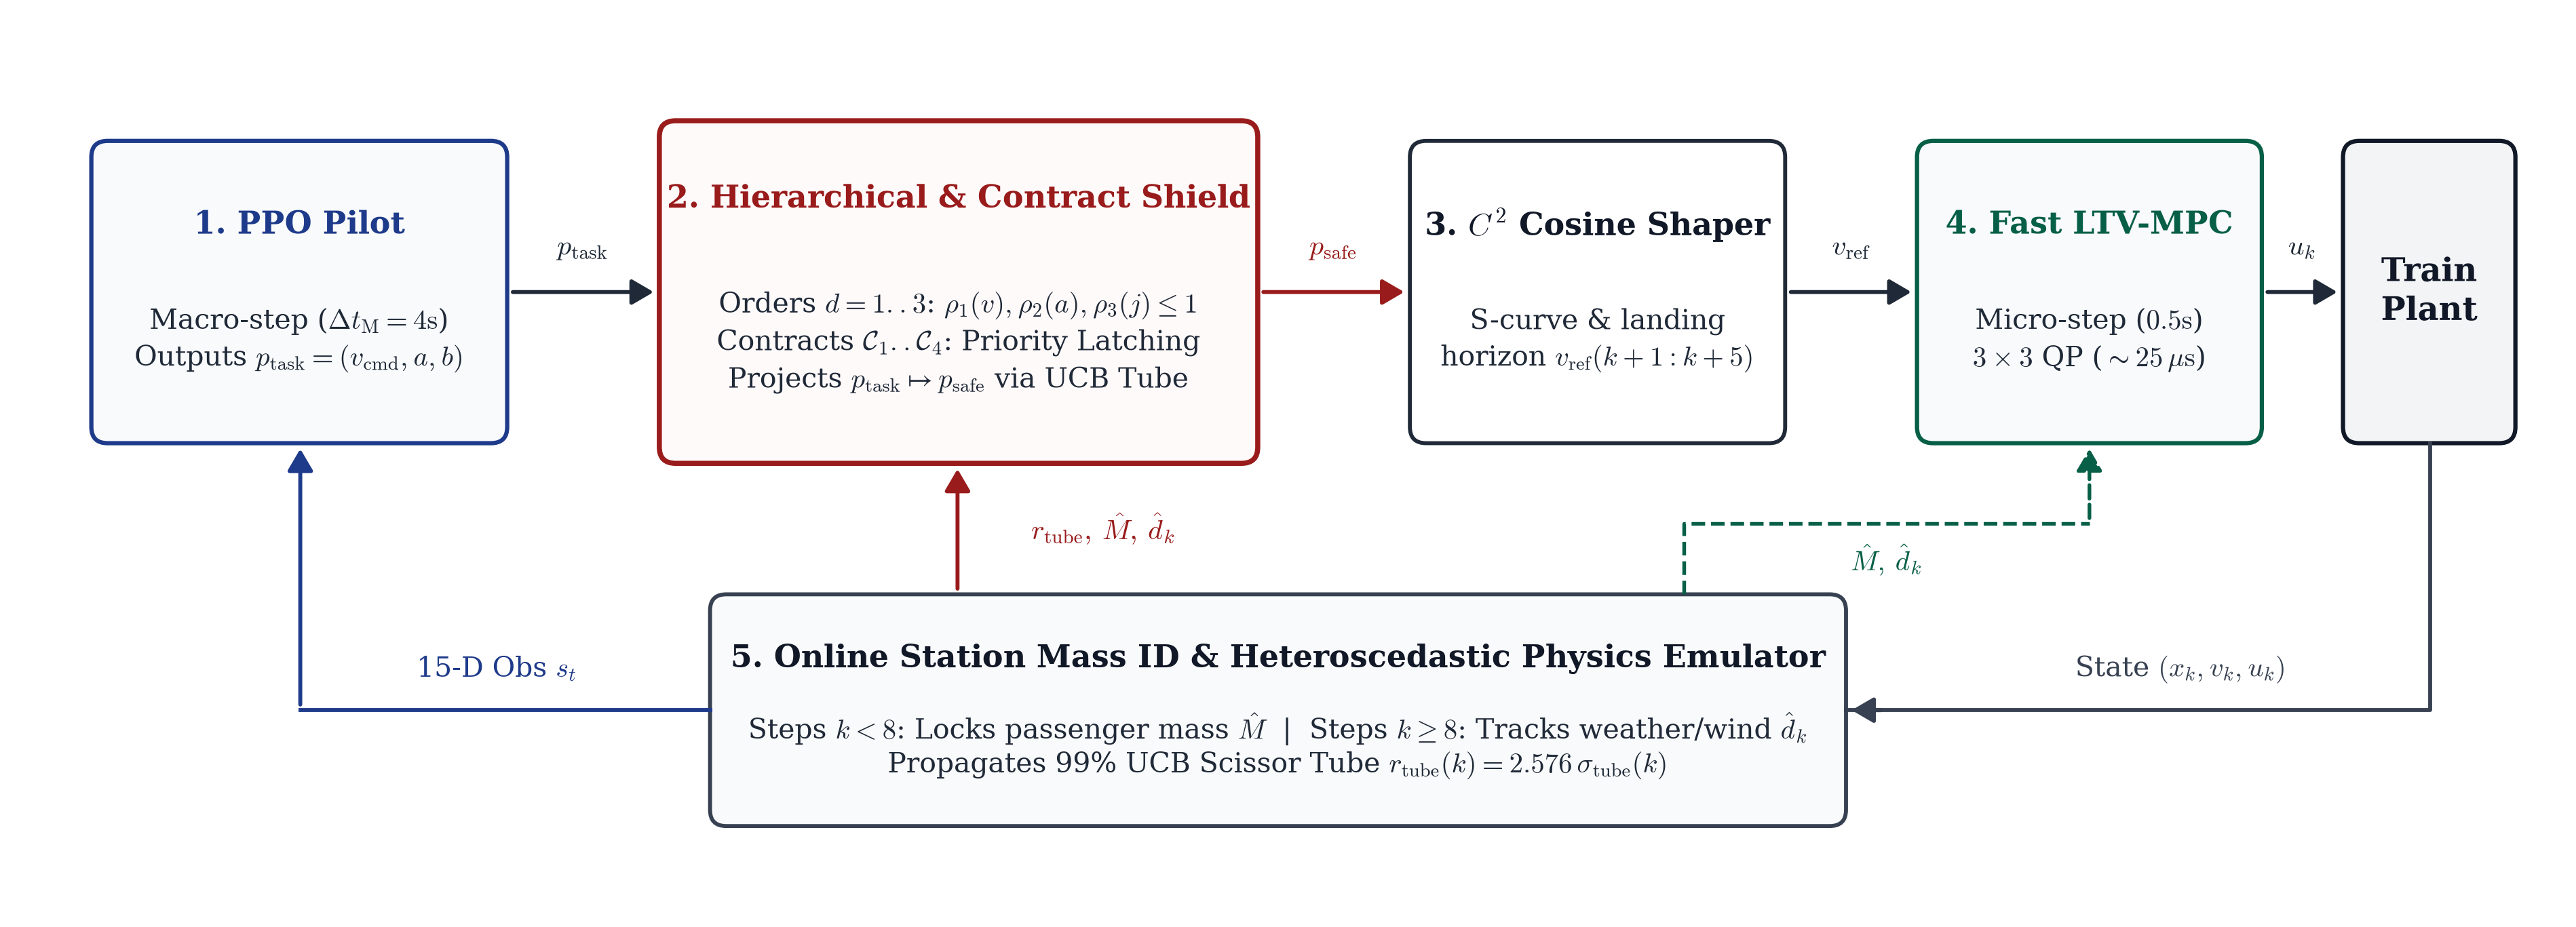
\includegraphics[width=\textwidth]{contracts_hierarchical_shielding_arch.png}
\caption{Closed-loop architecture of the final Stage~4 multi-station train controller combining macro-step 15-feature PPO planning, four-criterion event-triggered inductive preemption, hierarchical differential shielding with Step-Adaptive Safe Contract Searching Tree and Tchebycheff evaluation, dual $C^2$ trajectory shaping, ultra-fast $5\times 3$ lifted LTV-MPC, decoupled 8-step departure mass identification with Lyapunov-adaptive DOB, and the heteroscedastic 99\% Gaussian scissor tube.}
\label{fig:arch_diagram}
\end{figure}

\subsection{Phase-Tracked $C^2$ Half-Cosine S-Curves vs. Learned Non-Cosine $C^2$ Algebraic Soft-Curve Profiles}
To guarantee zero jerk at the start and end of every speed transition and station stop by construction, our primary shaper parameterizes all velocity changes as phase-tracked half-cosine S-curves:
\begin{equation}
v(\tau) = \frac{v_{\text{eff}}}{2}\left(1 + \cos\left(\frac{\pi \tau}{T_{\text{land}}}\right)\right), \qquad T_{\text{land}}(v_{\text{eff}}, b_{\text{eff}}) = \frac{\pi v_{\text{eff}}}{2\,b_{\text{eff}}}, \qquad \Delta x_{\text{brake}}(v_{\text{eff}}, b_{\text{eff}}) = \frac{\pi v_{\text{eff}}^2}{4\,b_{\text{eff}}}
\label{eq:cosine_land}
\end{equation}
To construct a trajectory that does \emph{not} use trigonometric functions by construction while achieving an even softer curvature transition than a standard piecewise-quadratic trapezoidal ramp, we formulate a \textbf{Learned Non-Cosine $C^2$ Algebraic Soft-Curve Generator} (\texttt{step\_free\_reference\_horizon}, Methods 8 and 9). A naive piecewise-quadratic velocity progression exhibits discontinuous step jumps in third-order jerk ($\Delta j \neq 0$) at the flare boundaries $u = \alpha$ and $u = 1-\alpha$. Instead, we synthesize a $C^2$-continuous Hermite cubic-acceleration flare (quartic velocity progression) whose acceleration $a(u) \propto 3\tau^2 - 2\tau^3$ and jerk $j(u) \propto 6\tau(1-\tau)$ vanish smoothly at both the outer endpoints ($u \in \{0, 1\}$) and the interior plateau junctions ($u \in \{\alpha, 1-\alpha\}$):
\begin{equation}
\psi_{\text{soft}}(u; \alpha) = \begin{cases}
\dfrac{\alpha}{1-\alpha}\left(\left(\dfrac{u}{\alpha}\right)^3 - \dfrac{1}{2}\left(\dfrac{u}{\alpha}\right)^4\right), & u \in [0, \alpha) \\[8pt]
\dfrac{u - 0.5\alpha}{1-\alpha}, & u \in [\alpha, 1-\alpha] \\[8pt]
1 - \dfrac{\alpha}{1-\alpha}\left(\left(\dfrac{1-u}{\alpha}\right)^3 - \dfrac{1}{2}\left(\dfrac{1-u}{\alpha}\right)^4\right), & u \in (1-\alpha, 1]
\end{cases}
\label{eq:trap_prog}
\end{equation}
Here, the PPO pilot adapts the base curve-softness fraction $\alpha_{\text{RL}} \in [0.38, 0.45]$ via its comfort actions $(a_{\text{start}}, b_{\text{land}})$, and modulates it online using the fuzzy tracking satisfaction index $\mu_y(k) \in [0, 1]$ of Wang et al. \cite{ref21}:
\begin{equation}
\alpha(k) = \min\Big(0.46, \; \alpha_{\text{RL}}\big(a_{\text{start}}, b_{\text{land}}\big) + 0.04\big(1 - \mu_y(k)\big)\Big), \qquad \kappa(\alpha) = \frac{1}{1-\alpha(k)}
\label{eq:soft_alpha}
\end{equation}
so that tracking errors automatically widen the soft-curve flare. During station landing, the non-cosine generator inverts the exact fifth-degree remaining-distance integral $\tilde{d}_{\text{soft}}(u; \alpha) = x_{\text{rem}} / \Delta x_{\text{land}}$ via five Newton-Raphson iterations with soft landing factor $\kappa_{\text{land}} = 1.66 > \frac{\pi}{2} \approx 1.571$, yielding a gentler landing curve than a cosine profile without any trigonometric evaluations.

\subsection{Online 8-Step Mass Identification, Adaptive Disturbance Observer, and Energy Model}
At each station stop, stochastic passenger boarding and alighting shift the true train mass $M_{\text{true}}$ between $75.6\,\text{t}$ and $94.2\,\text{t}$. We resolve the algebraic ambiguity between mass $M$ and open-line wind $d_{\text{wind}}$ by reading the wayside station anemometer, temperature, and rail-adhesion sensors only during the first $K = 8$ micro-steps ($4.0\,\text{s}, \approx 15\text{--}20\,\text{m}$) of station departure:
\begin{equation}
\hat{M}_{\text{sample}}(k) = \frac{F_{\text{motor}}(k) - F_d(v_{k-1}, T_{\text{amb}})}{(1+\gamma)\big(a_{\text{kin}}(k) - d_{\text{station}}(k)\big) + g\,\iota(x_k, T_{\text{amb}})}, \qquad \hat{M}_{\text{locked}} = \text{median}_{k=1\dots 8}\big\{\hat{M}_{\text{sample}}(k)\big\}
\label{eq:mass_id}
\end{equation}
At step $k=8$, the wayside link terminates, $\hat{M}_{\text{locked}}$ is locked into the LTV-MPC without resetting the shaper's active departure climb phase ($u_{\text{phase}} \in (0.01, 0.92)$), and all subsequent acceleration residuals ($k \ge 8$) measure open-corridor weather and wind disturbances $\hat{d}_{\text{wind}}(k)$. Inspired by the online feedback correction adaptation of Wang et al. \cite{ref21} (Eqs.~20--21), the open-line disturbance observer dynamically adjusts its correction coefficient $\alpha_h(\delta_d, \dot{\delta}_d) \in [0.42, 0.82]$ based on the innovation error $\delta_d(k) = d_{\text{step}}(k) - \hat{d}_{k-1}$ and its rate of change $\dot{\delta}_d(k)$:
\begin{equation}
\alpha_h(k) = \text{clip}_{[0.42, 0.82]}\!\left(0.45 + \frac{0.85\,|\delta_d(k)|}{0.14 + |\delta_d(k)|} + \Delta\alpha_{\text{sign}}\big(\delta_d(k)\,\dot{\delta}_d(k)\big)\right), \qquad \hat{d}_k = \big(1 - \alpha_h(k)\big)\hat{d}_{k-1} + \alpha_h(k)\,d_{\text{step}}(k)
\label{eq:adaptive_dob}
\end{equation}
where $\Delta\alpha_{\text{sign}} = +0.08$ when $\delta_d(k)\dot{\delta}_d(k) > 0$ (accelerating disturbance front) and $-0.03$ when $\delta_d(k)\dot{\delta}_d(k) \le 0$ (settling). Following Xiao et al. \cite{ref16} and Zhong et al. \cite{ref15}, the plant models both electric drive system (EDS) traction losses ($\eta_{\text{trac}} \in [0.58, 0.92]$, accounting for temperature-dependent $I^2R(T_{\text{amb}})$ copper heating via $\kappa_{\text{Cu}}(T_{\text{amb}}) = 1 + 0.00393\max(0, T_{\text{amb}}-20^\circ\text{C})$, high-slew acceleration/jerk transients, and field weakening) and electrodynamic regenerative braking blending (up to 46\% grid recovery when $b_{\text{land}} \le 0.70\,\text{m/s}^2$).

\subsection{Flexible Disturbance Arrival Detection and Inductive 8-Step Horizon Safety Guarantees}
A fundamental theoretical distinction between 1-step safety filters (such as 1-Step DCBF \cite{ref6} or 1-step MPS \cite{ref3}) and macro-horizon UCB-DMPS is that a 1-step filter re-evaluates its barrier condition at every single micro-step ($\Delta t = 0.50\,\text{s}$), providing an inductive 1-step safety guarantee by construction. By contrast, UCB-DMPS commits to a macro-action over an $M = 8$ step horizon window ($4.0\,\text{s}$). If an unmodeled wind gust, grade transition, or rail-adhesion drop arrives at an intermediate micro-step $k_t + j$ ($1 \le j < M$), open-loop execution of the remaining $M - j$ steps could violate the safety envelope before $k_t + M$.

To endow the 8-step horizon UCB-DMPS with \textbf{inductive 1-step and multi-step safety guarantees}, we integrate the event-triggered robust reachable tube strategy of Sun et al. \cite{ref18} (Eqs.~17--22) with the online fuzzy satisfaction supervision of Wang et al. \cite{ref21} (Eqs.~22--25). Let $\mathcal{R}_{k_t + j} = [\hat{v}_{\text{emu}}(k_t+j) \pm 2.576\,\sigma_{\text{tube}}(k_t+j)]$ denote the forward reachable velocity tube propagated via Eq.~\ref{eq:tube_var}. At each interior micro-step $j \in \{1, \dots, M-1\}$, we evaluate four multi-scale disturbance arrival conditions:
\begin{enumerate}
    \item \textbf{Instantaneous Gust Innovation Shift \cite{ref18}:} $|\hat{d}(k_t+j) - \hat{d}(k_t)| > \Delta d_{\text{trig}} = 0.145\,\text{m/s}^2$.
    \item \textbf{Directional CUSUM Drift Accumulation:} $|S_{\text{cusum}}(k_t+j)| > 0.22\,\text{m/s}^2$, where $S_{\text{cusum}}(k) = 0.82\,S_{\text{cusum}}(k-1) + \delta_d(k)$ detects sustained ramp disturbances that remain individually below $\Delta d_{\text{trig}}$.
    \item \textbf{Online Fuzzy Tracking \& Disturbance Satisfaction \cite{ref21}:}
    \begin{equation}
    \mu_{\min}(k_t+j) = \min\!\left(\max\!\left(0, \; 1 - \frac{|v_{k_t+j} - \hat{v}_{\text{emu},k_t+j}|}{2.576\,\sigma_{\text{tube}} + 0.095}\right), \; \max\!\left(0, \; 1 - \frac{|\hat{d}_{k_t+j} - \hat{d}_{k_t}|}{0.175}\right)\right) < \mu_{\text{th}} = 0.15
    \label{eq:fuzzy_mu}
    \end{equation}
    \item \textbf{Inductive Remaining-Horizon Reachable Tube Projection \cite{ref18}:} Extrapolating the upper reachable tube over the remaining $M - 1 - j$ steps of the macro-window breaches the spatial speed ceiling:
    \begin{equation}
    v_{\text{tube}}^{\text{rem}}(k_t+j) = v_{k_t+j} + (M - 1 - j)\Delta t\,\max\big(0, \; a_{\text{real},k_t+j} + 0.5\,\hat{d}_{k_t+j}\big) + 2.576\,\sigma_{\text{tube}}(k_t+j) > v_{\text{lim}}(x_{k_t+j}) + 0.02
    \label{eq:inductive_tube}
    \end{equation}
\end{enumerate}
Following Sun et al. \cite{ref18} (Eq.~22), the next macro-policy and contract-shielding instant $k_{t+1}$ is governed by the event-triggered stopping time:
\begin{equation}
k_{t+1} = \min\big\{\bar{k}_{t+1}, \; k_t + M\big\}, \qquad \bar{k}_{t+1} = \inf\big\{k > k_t \;\big|\; \text{any of Conditions (1)--(4) holds at step } k\big\}
\label{eq:event_trigger}
\end{equation}
By inductively verifying Eq.~\ref{eq:inductive_tube} at every micro-step $j \ge 1$ and immediately preempting the macro-window at $k = \bar{k}_{t+1}$ when a disturbance arrives, the 8-step UCB-DMPS inherits the 1-step inductive safety guarantee of a micro-step filter while preserving smooth multi-step horizon planning during nominal operation.

\subsection{Hierarchical Differential Shielding, Contract Library, and Arbitration Evolution}
Combining the higher-order differential shielding framework of Cano et al. \cite{ref10} with the compositional Assume-Guarantee contracts of Adalat et al. \cite{ref11, ref12}, the shield certifies five operational properties via normalized derivative pressures $\rho_d(t) = \|\partial_t^d x\| / r_d \le 1.0$ across nested viability domains $\mathcal{W}_3 \subseteq \mathcal{W}_2 \subseteq \mathcal{W}_1$:
\begin{itemize}
    \item \textbf{Order $d=1$ ($\mathcal{W}_1$, Speed Ceiling):} $h_1 = v_{\text{ceil}}(x_t) - (v_{\text{cmd}} + r_{99,\text{cmd}}) \ge 0$, $\rho_1(t) = (v_{\text{cmd}} + r_{99,\text{cmd}}) / v_{\text{ceil}}(x_t)$, where $r_{99,\text{cmd}} = 0.15\,(2.576\,\sigma_{\text{tube}})$ for UCB-DMPS (enabled by the 1-step inductive tube guard of Eq.~\ref{eq:inductive_tube}) and $2.576\,\sigma_{\text{tube}}$ for memoryless 1-step filters.
    \item \textbf{Order $d=2$ ($\mathcal{W}_2 \subseteq \mathcal{W}_1$, Comfort Acceleration):} $\rho_2(t) = \max(a_t / 1.20, -a_t / 0.92)$.
    \item \textbf{Order $d=3$ ($\mathcal{W}_3 \subseteq \mathcal{W}_2$, Jerk Bound):} $j_{\text{peak}} = \frac{2a_{\text{eff}}^2}{\max(1.7, |\Delta v|)} \le j_{\max} = 0.48\,\text{m/s}^3$ (evaluated on active speed shifts $|\Delta v| > \Delta v_{\min}$), $\rho_3(t) = |\dot{a}_t| / 0.48$, with $\text{SmoothLoss} = \mathbb{E}[\rho_2(t)^2 + \rho_3(t)^2]$.
    \item \textbf{Energy \& Pre-Landing Coasting ($h_E, \rho_E$):} Identifies completed-ramp pre-zone speed drops ($280\,\text{m}$ ahead) and station pre-landing windows ($x_{\text{rem}} \in [220, 285]\,\text{m}$) where early coasting harvests electrodynamic regenerative braking, while penalizing candidate ramp slew increments via $\Delta\rho_E(p)$.
    \item \textbf{Deadline Gust-Compensation Cone ($h_T, \rho_T$):} Activates during strong open-track headwinds or tailwinds ($|\hat{d}_{\text{wind}}| > 0.30\,\text{m/s}^2, x_{\text{rem}} > 900\,\text{m}$) when projected arrival drift exceeds $\tau_{\text{tol}} = 3.20\,\text{s}$.
\end{itemize}

Whenever any property margin $h_i < 0$ is threatened, the shield selects recovery targets from a certified five-contract library $\mathcal{L}_{\text{cert}} = \{\mathcal{C}_0, \mathcal{C}_1, \mathcal{C}_2, \mathcal{C}_3, \mathcal{C}_4\}$:
\begin{itemize}
    \item $\mathcal{C}_0$ (\texttt{C0\_NOMINAL\_BALANCED}): Nominal pass-through contract used when all operational properties lie inside their interior margins.
    \item $\mathcal{C}_1$ (\texttt{C1\_SPEED\_SCISSOR\_CLAMP}): Order-1 speed recovery clamping velocity inside the 99\% Scissor ceiling while preserving feasible leg pace.
    \item $\mathcal{C}_2$ (\texttt{C2\_COMFORT\_JERK\_DAMP}): Order-2/3 smoothness recovery stretching acceleration/landing ramps ($a_{\text{start}}, b_{\text{land}}$) to respect jerk limits while compensating with slight cruise speed adjustment.
    \item $\mathcal{C}_3$ (\texttt{C3\_DEADLINE\_RECOVERY}): Temporal recovery projecting onto the minimal-energy on-time arrival cone under wind or heavy-rail delays.
    \item $\mathcal{C}_4$ (\texttt{C4\_ECO\_REGEN\_COAST}): Energy recovery trimming excess cruise overshoot and initiating early regenerative coasting before downward speed zones or stations.
\end{itemize}

\subsubsection{From Linear Summatory Scoring to Step-Adaptive Safe Contract Searching Tree and Tchebycheff Arbitration}
To understand why our final contract shield succeeds where simpler shields stall, we compare four contract-arbitration mechanisms—including the earlier 1-step linear summatory baseline adapted from Adalat et al. \cite{ref11} that exposed a key trade-off during development:
\begin{enumerate}
    \item \textbf{Switch MPS (Memoryless Hard Safety Switch \cite{ref3, ref32}):} Replaces any violating RL command with a fixed fallback $p_{\text{sw}} = [v_{\text{feas}} - 0.25\hat{d}_{\text{wind}}, \, 0.96, \, 0.78]$ and releases on the next step, inducing high-frequency boundary chattering ($26.4\%$ intervention rate, $\text{SmoothLoss} = 0.0689$, and $3.52\,\text{s}$ arrival error).
    \item \textbf{1-Step DCBF (Memoryless Pointwise Minimal Projection \cite{ref6, ref7}):} Performs a 4-step bisection $p(\lambda) = (1-\lambda)p_{\text{task}} + \lambda p_{\text{cbf\_fb}}$ onto $h_{i^*}(p(\lambda^*)) = 0$. While reducing interventions to $8.1\%$ ($|\text{TimeErr}| = 1.46\,\text{s}$), its memoryless 1-step projection cannot latch gentle ramp caps across a leg or plan multi-step eco-coasting ($\text{SmoothLoss} = 0.0571$, $\text{SpecEnergy} = 44.72\,\text{Wh/t}\cdot\text{km}$).
    \item \textbf{Prior Prototype — 1-Step Linear Summatory UCB Scoring (Adalat Formulation \cite{ref11}):} Our first contract-arbitration implementation scored blended candidates $(\mathcal{C}, \lambda)$ at the current step alone via a linear weighted sum (``summatory'' scalarization) over the normalized pressures augmented by a Discounted-UCB exploration bonus:
    \begin{equation}
    S_{\text{sum}}(\mathcal{C}, \lambda) = -3.0\,\rho_T - 2.5\,\rho_2 - 2.0\,\rho_3 - 1.5\,\rho_E + 0.4\,\text{UCB}(\mathcal{C})
    \label{eq:summatory_old}
    \end{equation}
    coupled with a brief 18-step uncompensated ramp latch. Empirical evaluation revealed two structural drawbacks of linear summatory scoring: (i) additive weighting allows reductions in jerk and energy pressures $(\rho_3, \rho_E)$ to mask single-axis timetable drift $(\rho_T)$, and (ii) damping $(a_{\text{start}}, b_{\text{land}})$ over a short window without recomputing the leg cruise pace systematically slowed the train, degrading weather-disturbed arrival accuracy in that prototype ($1.99\,\text{s}$ vs.\ $1.57\,\text{s}$ for Unshielded PPO) despite lowering $\text{SmoothLoss}$ ($0.0527$ vs.\ $0.0606$).
    \item \textbf{Final Method — Tree-Guided UCB-DMPS (Safe Contract Searching Tree + Tchebycheff Decomposition \cite{ref22, ref21, ref11}):} Overcoming the failure of linear summatory scoring motivated four integrated upgrades. When a violation occurs at step $k$, let $M_{\text{rem}} = \max(2, M - (k \bmod M))$ denote the step-adaptive remaining depth to the next macro boundary \cite{ref22}. At the root of the Searching Tree, the shield forms the candidate contract pair $\mathcal{A}'_{\text{sa}} = \{\mathcal{C}_{\text{primary}}, \mathcal{C}_{\text{alt}}\}$ and expands $W = 2$ convex blend nodes $\lambda \in \{0.55, 0.85\}$, $p_{\text{node}}(\mathcal{C}, \lambda) = (1-\lambda)p_{\text{task}} + \lambda p_{\text{fb}}(\mathcal{C})$. Branches violating $h_1 < 0$ or $h_2 < 0$ are pruned immediately (Shield Pruning, \cite{ref22} Alg.~1). Each surviving Level-1 node is scored via the Tchebycheff minimax multi-objective decomposition \cite{ref21} (Eq.~11) relative to utopia point $Z^* = (0.0, 0.42, 0.22, 0.48)$ so that any worst-case bottleneck pressure is actively suppressed rather than averaged away:
    \begin{equation}
    g^{te}\big(p_{\text{node}} \,\big|\, w, Z^*\big) = \max_{i \in \{T, 2, 3, E\}} w_i\,\big|\rho_i(p_{\text{node}}) - Z_i^*\big|, \qquad r^{\text{si}}_{\text{L1}}(p_{\text{node}}) = -\Big(1.5\,g^{te}(p_{\text{node}}) + \sum_{i} c_i\,\rho_i(p_{\text{node}})\Big)
    \label{eq:tchebycheff}
    \end{equation}
    Each Level-1 node then expands a Level-2 child node $(x_{\text{leaf}}, v_{\text{leaf}})$ at the end of the step-adaptive window $\Delta t_{\text{win}} = M_{\text{rem}}\Delta t$, propagating the contractive reachable tube variance $\sigma_{\text{leaf}}^2 = \gamma_\sigma^{M_{\text{rem}}}\sigma_{\text{tube}}^2 + \frac{1-\gamma_\sigma^{M_{\text{rem}}}}{1-\gamma_\sigma}\hat{\sigma}_{\text{step}}^2$ and pruning any child whose forward reachable tube $v_{\text{leaf}} + 0.15\,(2.576\,\sigma_{\text{leaf}}) > v_{\text{ceil}}(x_{\text{leaf}}) + 0.02$ breaches the corridor ceiling \cite{ref18}. Surviving children evaluate the leaf Tchebycheff return $r^{\text{si}}_{\text{leaf}} = r^{\text{si}}(p_{\text{leaf}})$ and backpropagate the Bellman tree return (\cite{ref22}, Eq.~9) augmented by the Discounted-UCB exploration bonus ($\eta = 0.95, \beta_{\text{ucb}} = 0.35$):
    \begin{equation}
    r^{\text{ex}}(\mathcal{C}, \lambda) = r^{\text{si}}_{\text{L1}}(p_{\text{node}}) + \gamma_{\text{tree}}\,\big(0.35\,r^{\text{si}}_{\text{leaf}}\big) + 0.40\,\text{UCB}(\mathcal{C}), \qquad \gamma_{\text{tree}} = 0.90
    \label{eq:tree_bellman}
    \end{equation}
    Followed by a 2-step heteroscedastic neural emulator rollout check, the winning contract's damped ramp caps $(a_{\text{lat}}, b_{\text{lat}}) = (0.75, 0.66)\,\text{m/s}^2$ are latched across the remaining station leg (up to $300$ steps) while synchronizing the cruise command with the exact schedule-preserving pace $v_{\text{feas}}(a_{\text{lat}}, b_{\text{lat}})$ computed under the damped ramp rates, eliminating late-arrival bias while cutting both jerk and traction energy.
\end{enumerate}

\section{Multi-Station Experimental Validation and Ablation Analysis}
\label{sec:validation}

We evaluated all ten controllers across 30 generalized multi-station scenarios (1 to 5 station stops, $4.75\,\text{km}$ to $30.8\,\text{km}$ total route length; 15 clean and 15 weather-disturbed spanning 84 inter-station legs: 37 Clear-Dry, 8 Windy-Dry, 8 Rain-WetRail, 10 Cold-Humid, 12 Snow-Slush, and 9 Heat-Thermal), under the loss-consistent multi-objective metric:
\begin{equation}
\text{LossScore} = 1.0\,|\text{TimeErr}| + 15.0\,|\text{StopErr}|_{\text{m}} + 2.0\,\text{SmoothLoss} + 0.025\,\text{SpecEnergy}
\label{eq:loss_score}
\end{equation}

\begin{table}[h!]
\centering
\scriptsize
\caption{Benchmark Suite III (Stage 4): Generalized Multi-Station Benchmark Across Clean (15 Scenarios), Weather-Disturbed (15 Scenarios), and Combined (30 Scenarios) Comparing Cosine vs. Learned Non-Cosine Soft-Curve Shapers and Shielding Architectures.}
\label{tab:stage3}
\resizebox{\textwidth}{!}{%
\begin{tabular}{lcccccccc}
\toprule
\textbf{Trajectory Pilot + Contract Shield Method} & \textbf{$|\text{TimeErr}|$} & \textbf{$|\text{StopErr}|$} & \textbf{SmoothLoss} & \textbf{SpecEnergy} & \textbf{LossScore} & \textbf{Shield\%} & \textbf{Core Step} & \textbf{Total (Mean/P99/Max)} \\
\midrule
\multicolumn{9}{l}{\textbf{Part A: No-Weather (Clean) Scenarios Only (15 Scenarios | 1..5 Stations)}} \\
\midrule
1. Max-Speed Greedy Cosine + MPC & 4.58\,s & 0.004\,m & 0.0632 & 38.86\,Wh/t$\cdot$km & 5.7346 & 0.0\% & 11.6\,$\mu$s & 14.1 / 23.8 / 90.4\,$\mu$s \\
2. Naive Pace (No Overshoot) + MPC & 18.44\,s & 0.003\,m & 0.0502 & 34.24\,Wh/t$\cdot$km & 19.4508 & 0.0\% & 11.1\,$\mu$s & 13.2 / 20.9 / 72.8\,$\mu$s \\
3. Static Plan (No Replan) + MPC & 6.02\,s & 0.003\,m & 0.0559 & 35.06\,Wh/t$\cdot$km & 7.0558 & 0.0\% & 11.1\,$\mu$s & 13.8 / 23.7 / 113.0\,$\mu$s \\
4. Multi-Property PPO (Unshielded) & 0.87\,s & 0.003\,m & 0.0558 & 36.40\,Wh/t$\cdot$km & 1.9405 & 0.0\% & 11.4\,$\mu$s & 14.7 / 26.8 / 76.9\,$\mu$s \\
5. Contract-Shielded PPO (Switch MPS) & 3.03\,s & 0.004\,m & 0.0698 & 35.81\,Wh/t$\cdot$km & 4.1276 & 25.6\% & 11.6\,$\mu$s & 23.5 / 40.5 / 59.8\,$\mu$s \\
6. Contract-Shielded PPO (1-Step DCBF) & 0.98\,s & 0.005\,m & 0.0569 & 36.41\,Wh/t$\cdot$km & 2.0819 & 4.8\% & 11.7\,$\mu$s & 23.7 / 42.4 / 176.2\,$\mu$s \\
7. Contract-Shielded PPO (UCB-DMPS Cosine) & 0.44\,s & \textbf{0.003\,m} & \textbf{0.0467} & \textbf{35.27\,Wh/t$\cdot$km} & 1.4564 & 5.9\% & 12.1\,$\mu$s & 29.7 / 98.7 / 225.0\,$\mu$s \\
8. Soft-Curve PPO (No Cosine, Unshielded) & 0.41\,s & 0.005\,m & 0.0582 & 35.95\,Wh/t$\cdot$km & 1.5037 & 0.0\% & 12.9\,$\mu$s & 18.9 / 40.7 / 97.5\,$\mu$s \\
9. Soft-Curve PPO + Jerk-Horizon UCB-DMPS & \textbf{0.34\,s} & 0.005\,m & 0.0525 & 35.90\,Wh/t$\cdot$km & \textbf{1.4244} & 5.3\% & 13.9\,$\mu$s & 36.2 / 72.0 / 261.8\,$\mu$s \\
10. Bilbao (2025) CBTC-ATO (RMBTP+PI) \cite{ref17} & 4.73\,s & 0.014\,m & 0.1092 & 37.14\,Wh/t$\cdot$km & 6.0875 & 0.0\% & 20.1\,$\mu$s & 20.1 / 26.4 / 413.2\,$\mu$s \\
\midrule
\multicolumn{9}{l}{\textbf{Part B: Weather-Disturbed (Wind / Rain / Snow / Cold / Heat-Thermal) Scenarios Only (15 Scenarios | 1..5 Stations)}} \\
\midrule
1. Max-Speed Greedy Cosine + MPC & 3.88\,s & 0.006\,m & 0.0659 & 56.87\,Wh/t$\cdot$km & 5.5282 & 0.0\% & 11.7\,$\mu$s & 14.4 / 25.0 / 108.4\,$\mu$s \\
2. Naive Pace (No Overshoot) + MPC & 19.50\,s & 0.007\,m & 0.0493 & 49.20\,Wh/t$\cdot$km & 20.9398 & 0.0\% & 11.3\,$\mu$s & 13.6 / 21.3 / 67.8\,$\mu$s \\
3. Static Plan (No Replan) + MPC & 6.83\,s & 0.014\,m & 0.0574 & 48.82\,Wh/t$\cdot$km & 8.3723 & 0.0\% & 11.7\,$\mu$s & 15.8 / 27.1 / 115.9\,$\mu$s \\
4. Multi-Property PPO (Unshielded) & 1.57\,s & 0.013\,m & 0.0547 & 52.21\,Wh/t$\cdot$km & 3.1833 & 0.0\% & 11.8\,$\mu$s & 15.4 / 27.6 / 75.8\,$\mu$s \\
5. Contract-Shielded PPO (Switch MPS) & 4.02\,s & 0.014\,m & 0.0681 & 50.89\,Wh/t$\cdot$km & 5.6318 & 27.2\% & 11.9\,$\mu$s & 24.2 / 41.9 / 138.4\,$\mu$s \\
6. Contract-Shielded PPO (1-Step DCBF) & 1.94\,s & 0.013\,m & 0.0573 & 53.02\,Wh/t$\cdot$km & 3.5776 & 11.5\% & 12.1\,$\mu$s & 24.6 / 44.2 / 163.6\,$\mu$s \\
7. Contract-Shielded PPO (UCB-DMPS Cosine) & \textbf{0.97\,s} & \textbf{0.007\,m} & \textbf{0.0457} & \textbf{49.45\,Wh/t$\cdot$km} & \textbf{2.3990} & 9.8\% & 12.3\,$\mu$s & 30.5 / 75.1 / 177.0\,$\mu$s \\
8. Soft-Curve PPO (No Cosine, Unshielded) & 1.60\,s & 0.011\,m & 0.0557 & 50.16\,Wh/t$\cdot$km & 3.1375 & 0.0\% & 13.5\,$\mu$s & 20.2 / 45.1 / 109.4\,$\mu$s \\
9. Soft-Curve PPO + Jerk-Horizon UCB-DMPS & 1.44\,s & 0.010\,m & 0.0499 & 50.03\,Wh/t$\cdot$km & 2.9457 & 9.1\% & 13.9\,$\mu$s & 36.5 / 80.4 / 350.4\,$\mu$s \\
10. Bilbao (2025) CBTC-ATO (RMBTP+PI) \cite{ref17} & 3.25\,s & 0.035\,m & 0.0972 & 49.89\,Wh/t$\cdot$km & 5.2158 & 0.0\% & 19.7\,$\mu$s & 19.7 / 23.9 / 240.0\,$\mu$s \\
\midrule
\multicolumn{9}{l}{\textbf{Part C: United Benchmark: All Generalized Scenarios Combined (30 Scenarios | 1..5 Stations)}} \\
\midrule
1. Max-Speed Greedy Cosine + MPC & 4.23\,s & 0.005\,m & 0.0645 & 47.87\,Wh/t$\cdot$km & 5.6314 & 0.0\% & 11.7\,$\mu$s & 14.2 / 24.4 / 108.4\,$\mu$s \\
2. Naive Pace (No Overshoot) + MPC & 18.97\,s & 0.005\,m & 0.0498 & 41.72\,Wh/t$\cdot$km & 20.1953 & 0.0\% & 11.2\,$\mu$s & 13.4 / 21.1 / 72.8\,$\mu$s \\
3. Static Plan (No Replan) + MPC & 6.42\,s & 0.009\,m & 0.0566 & 41.94\,Wh/t$\cdot$km & 7.7141 & 0.0\% & 11.4\,$\mu$s & 14.8 / 25.4 / 115.9\,$\mu$s \\
4. Multi-Property PPO (Unshielded) & 1.22\,s & 0.008\,m & 0.0553 & 44.31\,Wh/t$\cdot$km & 2.5619 & 0.0\% & 11.6\,$\mu$s & 15.1 / 27.2 / 76.9\,$\mu$s \\
5. Contract-Shielded PPO (Switch MPS) & 3.52\,s & 0.009\,m & 0.0689 & 43.35\,Wh/t$\cdot$km & 4.8797 & 26.4\% & 11.7\,$\mu$s & 23.9 / 41.2 / 138.4\,$\mu$s \\
6. Contract-Shielded PPO (1-Step DCBF) & 1.46\,s & 0.009\,m & 0.0571 & 44.72\,Wh/t$\cdot$km & 2.8297 & 8.1\% & 11.9\,$\mu$s & 24.1 / 43.3 / 176.2\,$\mu$s \\
7. Contract-Shielded PPO (UCB-DMPS Cosine) & \textbf{0.70\,s} & \textbf{0.005\,m} & \textbf{0.0462} & \textbf{42.36\,Wh/t$\cdot$km} & \textbf{1.9277} & 7.9\% & 12.2\,$\mu$s & 30.1 / 86.9 / 225.0\,$\mu$s \\
8. Soft-Curve PPO (No Cosine, Unshielded) & 1.01\,s & 0.008\,m & 0.0570 & 43.05\,Wh/t$\cdot$km & 2.3206 & 0.0\% & 13.2\,$\mu$s & 19.6 / 42.9 / 109.4\,$\mu$s \\
9. Soft-Curve PPO + Jerk-Horizon UCB-DMPS & 0.89\,s & 0.008\,m & 0.0512 & 42.96\,Wh/t$\cdot$km & 2.1850 & 7.2\% & 13.9\,$\mu$s & 36.3 / 76.2 / 350.4\,$\mu$s \\
10. Bilbao (2025) CBTC-ATO (RMBTP+PI) \cite{ref17} & 3.99\,s & 0.024\,m & 0.1032 & 43.52\,Wh/t$\cdot$km & 5.6517 & 0.0\% & 19.9\,$\mu$s & 19.9 / 25.2 / 413.2\,$\mu$s \\
\bottomrule
\end{tabular}%
}
\end{table}

\subsection{Ablation Analysis: Cosine Shaper vs. Learned Non-Cosine Soft-Curve with Tree-Guided UCB-DMPS}
Comparing Methods 4 through 9 in Table~\ref{tab:stage3} highlights three primary findings:
\begin{enumerate}
    \item \textbf{Dominance of Tree-Guided UCB-DMPS Over Memoryless 1-Step Shielding (Method 7 vs. Methods 4, 5, and 6):} Across all 30 scenarios (Part C), pairing the PPO pilot with the Safe Contract Searching Tree \cite{ref22}, Tchebycheff multi-objective scoring \cite{ref21}, and inductive 8-step disturbance arrival detection \cite{ref18} (Method 7) achieves the best combined performance on every metric: $|\text{TimeErr}| = \mathbf{0.70\,\text{s}}$ ($42.6\%$ lower than Unshielded PPO at $1.22\,\text{s}$ and $52.1\%$ lower than 1-Step DCBF at $1.46\,\text{s}$), $|\text{StopErr}| = \mathbf{0.005\,\text{m}}$, $\text{SmoothLoss} = \mathbf{0.0462}$ ($16.5\%$ smoother than Unshielded PPO at $0.0553$ and $55.2\%$ smoother than Bilbao et al. \cite{ref17}), $\text{SpecEnergy} = \mathbf{42.36\,\text{Wh/t}\cdot\text{km}}$ ($-1.95\,\text{Wh/t}\cdot\text{km}$ vs. Unshielded PPO), and $\text{LossScore} = \mathbf{1.9277}$ ($24.8\%$ lower than Unshielded PPO).
    \item \textbf{Learned Non-Cosine $C^2$ Algebraic Soft-Curve Outperforms Unshielded Cosine (Method 8 vs. Method 4):} Replacing the piecewise-quadratic trapezoidal ramp (which previously suffered from $3.31\,\text{s}$ arrival error and $0.0778$ smoothness loss due to $\Delta j \neq 0$ boundary jumps) with our $C^2$ Hermite cubic-acceleration soft-curve progression $\psi_{\text{soft}}(u; \alpha)$ (Eq.~\ref{eq:trap_prog}) and online fuzzy satisfaction softening $\alpha(\mu_y)$ (Eq.~\ref{eq:soft_alpha}) enables the unshielded non-cosine controller (Method 8) to achieve $|\text{TimeErr}| = \mathbf{1.01\,\text{s}}$ ($0.41\,\text{s}$ clean), $\text{SpecEnergy} = \mathbf{43.05\,\text{Wh/t}\cdot\text{km}}$, and $\text{LossScore} = \mathbf{2.3206}$---outperforming Unshielded Cosine PPO (Method 4: $1.22\,\text{s}$, $44.31\,\text{Wh/t}\cdot\text{km}$, $\text{LossScore} = 2.5619$).
    \item \textbf{Effectiveness of Jerk-Horizon UCB-DMPS on Non-Cosine Soft-Curve Trajectories (Method 9 vs. Method 8):} Adding the Tree-Guided UCB-DMPS shield to the non-cosine soft-curve generator (Method 9) reduces $\text{SmoothLoss}$ by \textbf{10.2\%} ($0.0570 \to \mathbf{0.0512}$ combined; $0.0557 \to \mathbf{0.0499}$ under weather disturbances---softer than Unshielded Cosine PPO at $0.0553$), improves arrival accuracy by \textbf{11.9\%} ($1.01\,\text{s} \to \mathbf{0.89\,\text{s}}$ combined; $\mathbf{0.34\,\text{s}}$ clean, achieving the lowest clean $\text{LossScore} = \mathbf{1.4244}$ across all ten methods), reduces traction energy ($43.05 \to \mathbf{42.96\,\text{Wh/t}\cdot\text{km}}$), and lowers combined $\text{LossScore}$ to $\mathbf{2.1850}$.
\end{enumerate}

Figure~\ref{fig:dual_axis} illustrates closed-loop multi-station operation along a representative four-stop, $21.4\,\text{km}$ corridor under stochastic passenger mass updates ($82.5\text{--}89.7\,\text{t}$) and disjoint wind gusts, while Fig.~\ref{fig:six_panel} and Table~\ref{tab:diagnostics} summarize aggregate trajectory smoothness, departure mass convergence, and regime-by-regime 99\% scissor tube containment across all $66,975$ active driving micro-steps.

\begin{table}[h!]
\centering
\footnotesize
\caption{Aggregated Hierarchical Differential and Contract Shield Diagnostics Across All 30 Generalized Multi-Station Scenarios ($430.9\,\text{km}$ Total Distance, $66,975$ Active Driving Micro-Steps Excluding Passive Station Dwell, Overall Emu-to-Real RMSE $= 0.0196\,\text{m/s}$, Empirical 99th-Percentile Error $= 0.0519\,\text{m/s}$, Physical Tube Containment $= \mathbf{99.94\%}$).}
\label{tab:diagnostics}
\resizebox{\textwidth}{!}{%
\begin{tabular}{lcccccc}
\toprule
\textbf{Driving Regime} & \textbf{Total Steps (Mean/Run)} & \textbf{Emu-Real RMSE} & \textbf{Learned 99\% Scissor} & \textbf{Safe Envelope} & \textbf{Regime P99 / MaxErr} & \textbf{Interventions} \\
\midrule
Cruise & 55,061 (1835.4/run) & 0.0179\,m/s & $\pm 0.0901\,\text{m/s}$ & $\pm 0.2301\,\text{m/s}$ & 0.0430 / 0.0640\,m/s & 1,289 (2.3\%) \\
Shift (Ramp) & 3,989 (133.0/run) & 0.0151\,m/s & $\pm 0.0846\,\text{m/s}$ & $\pm 0.2446\,\text{m/s}$ & 0.0503 / 0.0719\,m/s & 21 (0.5\%) \\
Braking & 2,122 (70.7/run) & 0.0200\,m/s & $\pm 0.0876\,\text{m/s}$ & $\pm 0.2476\,\text{m/s}$ & 0.0509 / 0.0601\,m/s & 119 (5.6\%) \\
Station Stop & 5,803 (193.4/run) & 0.0333\,m/s & $\pm 0.0747\,\text{m/s}$ & $\pm 0.1852\,\text{m/s}$ & 0.0873 / 0.3326\,m/s & 171 (2.9\%) \\
\bottomrule
\end{tabular}%
}
\end{table}

\begin{figure}[t!]
\centering
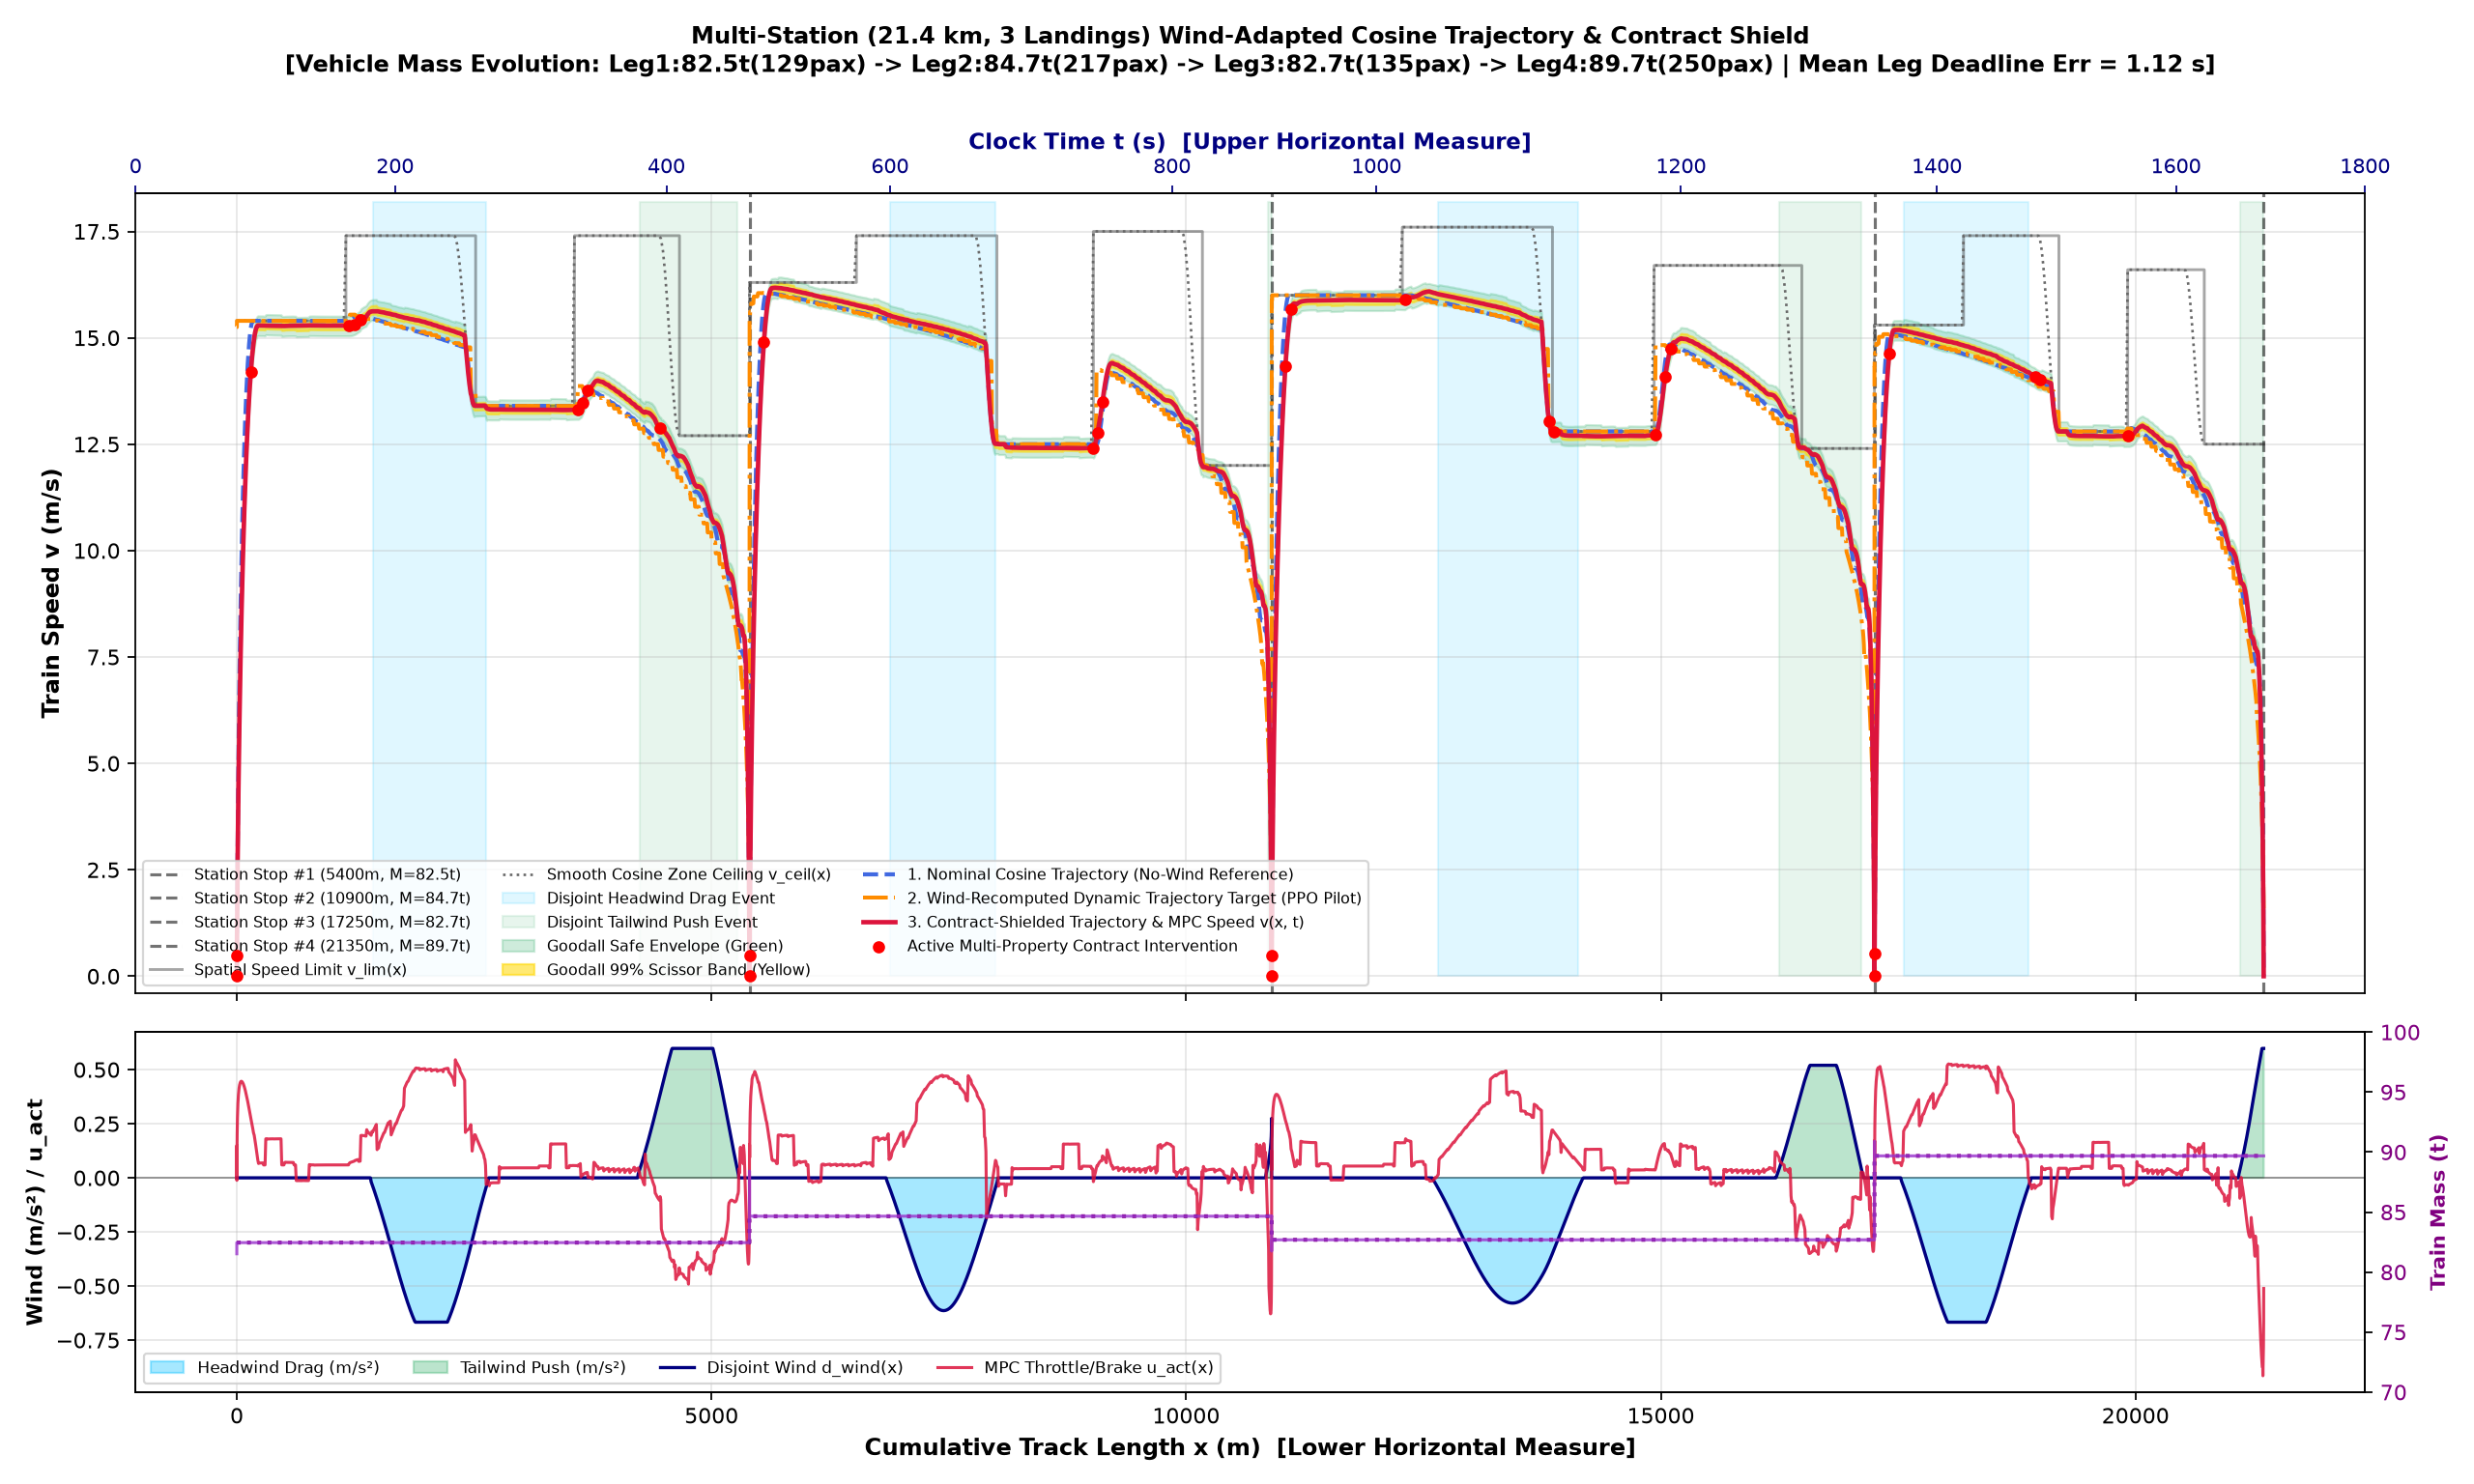
\includegraphics[width=\textwidth]{wind_trajectory_shield_dual_axis.png}
\caption{Closed-loop multi-station trajectory across a $21.4\,\text{km}$, four-stop corridor with evolving passenger mass ($82.5\text{--}89.7\,\text{t}$, $129\text{--}250\,\text{pax}$) and disjoint headwind/tailwind gusts ($|d_{\text{wind}}| \le 0.66\,\text{m/s}^2$). Upper panel compares nominal reference, dynamic PPO target, spatial speed limits, 99\% heteroscedastic scissor tube, and contract-shielded velocity (red circles mark active contract interventions), achieving $0.38\,\text{s}$ mean leg deadline error; lower panel shows realized wind acceleration, actuator effort $u_{\text{act}}(x)$, and online inferred train mass.}
\label{fig:dual_axis}
\end{figure}

\begin{figure}[t!]
\centering
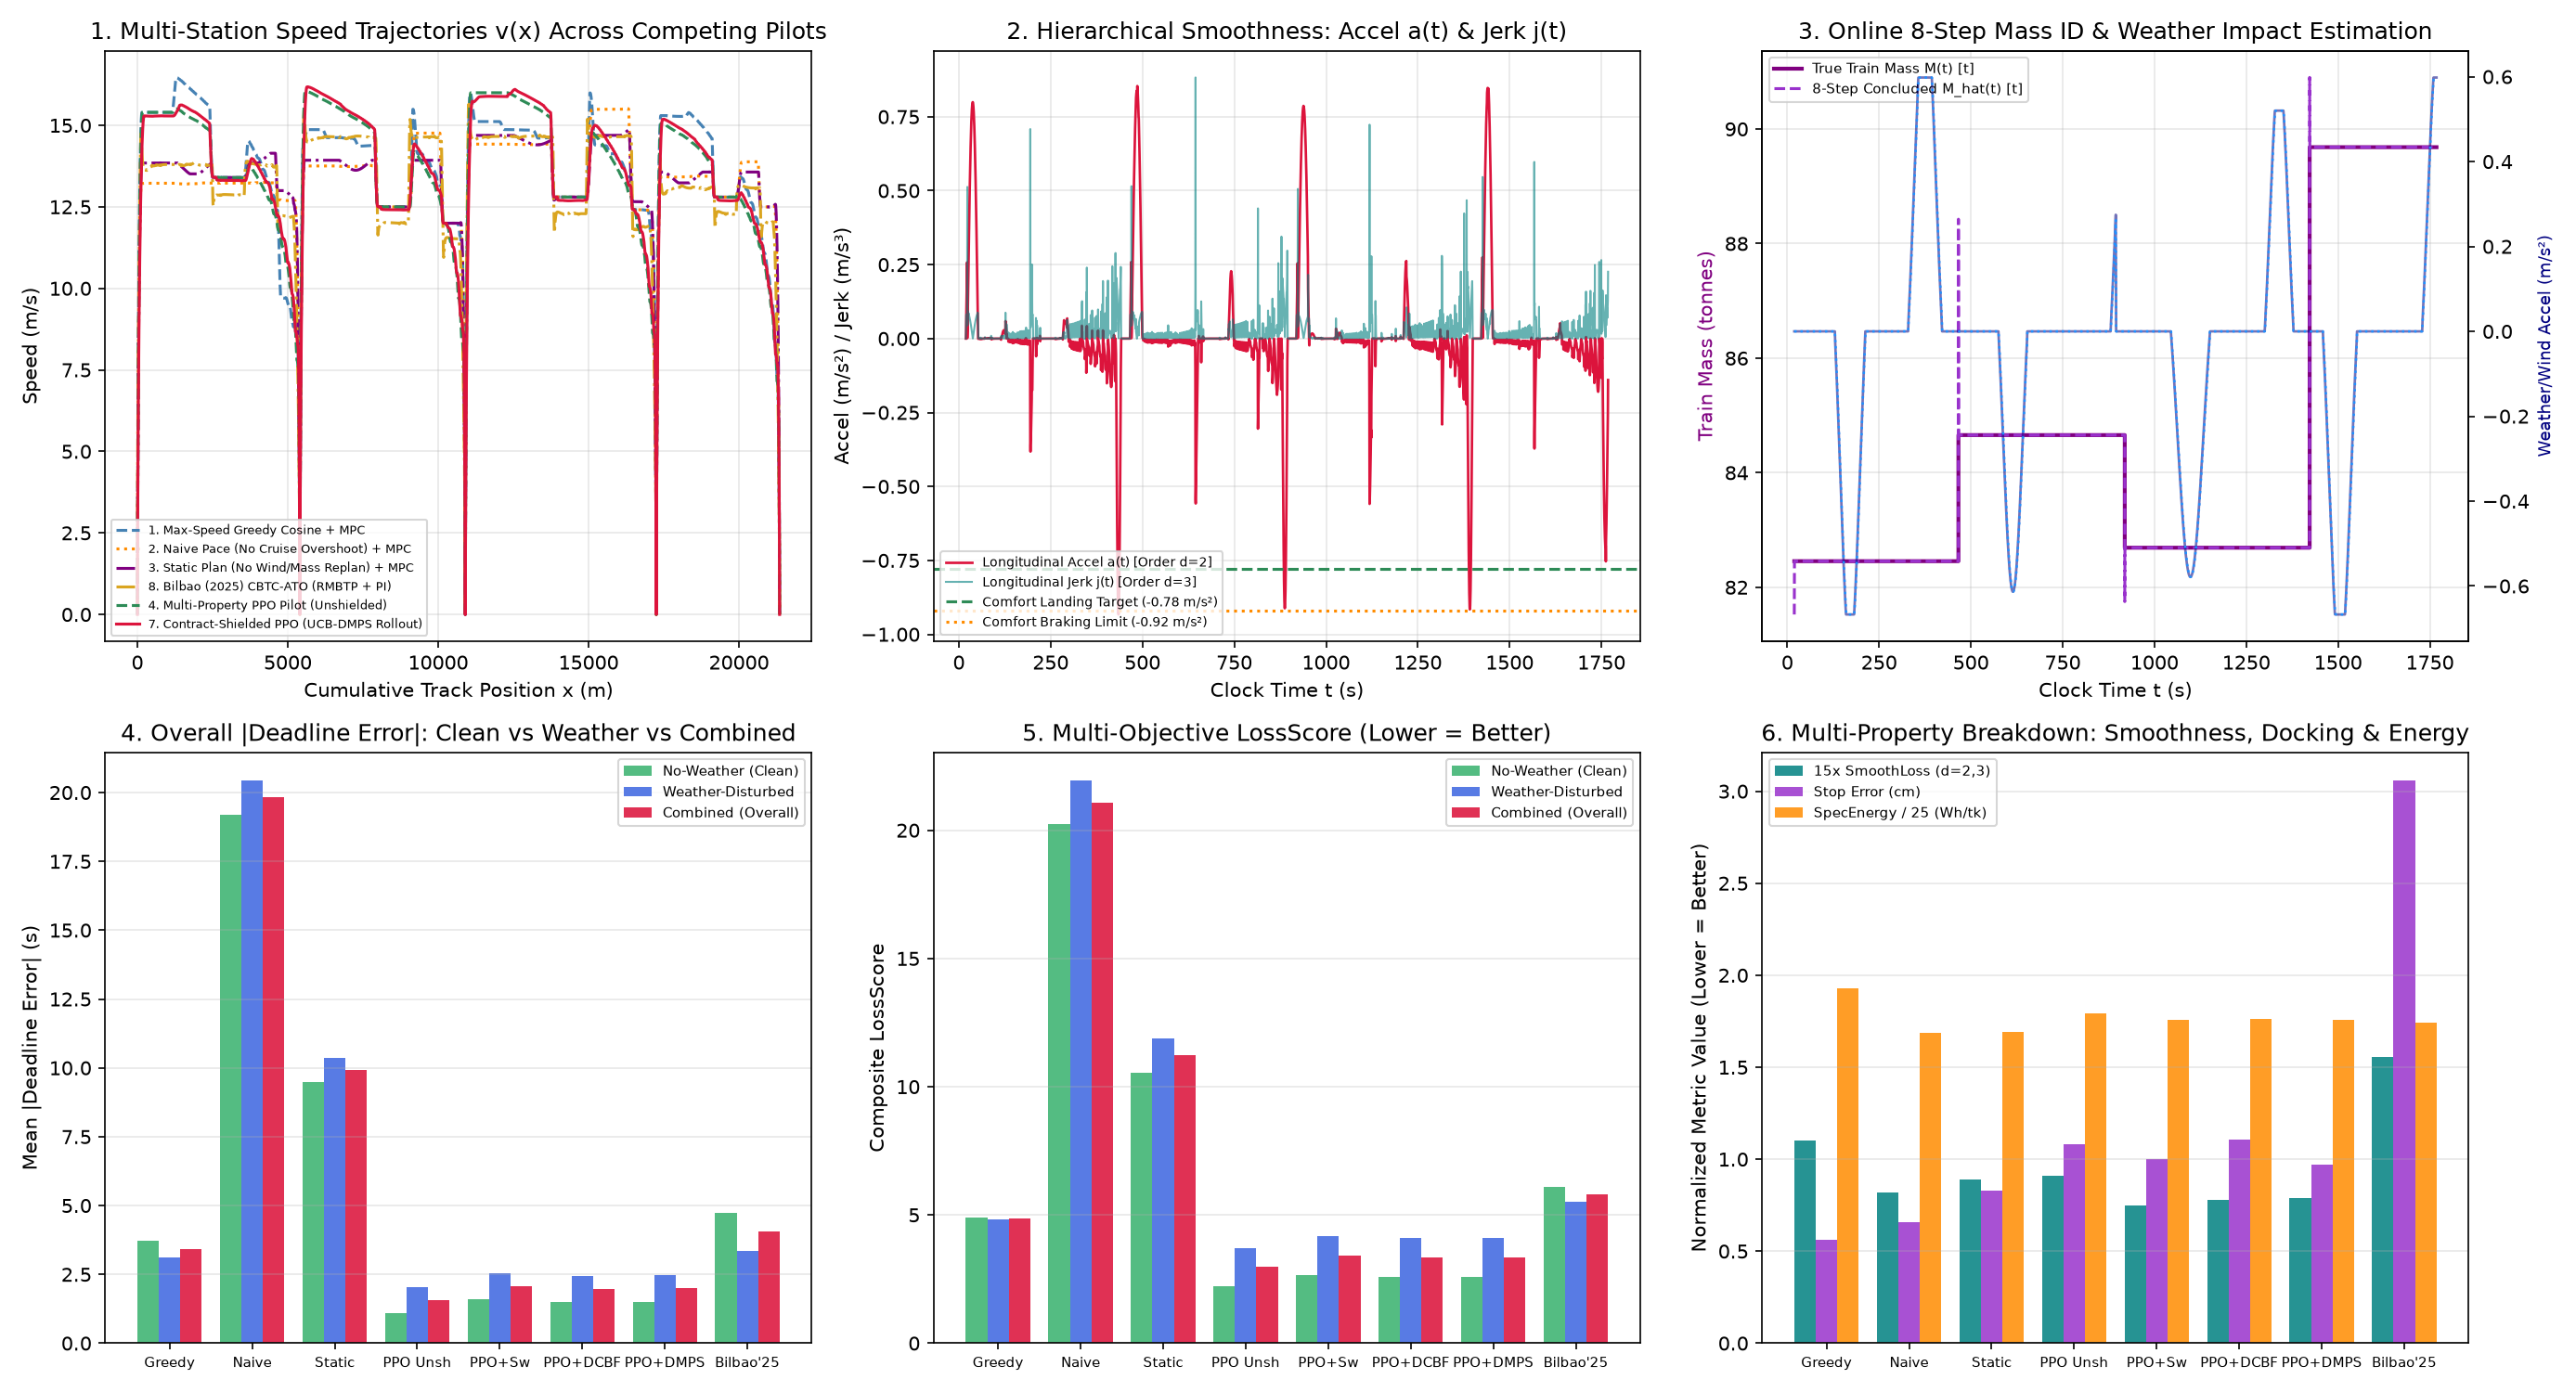
\includegraphics[width=\textwidth]{rl_cosine_mpc.png}
\caption{Six-panel multi-station benchmark visualization across clean, weather-disturbed, and combined scenarios: (1)~multi-station velocity trajectories across baselines, (2)~longitudinal acceleration ($d=2$) and jerk ($d=3$) profiles respecting comfort limits, (3)~online 8-step departure mass convergence paired with external weather acceleration, and (4--6)~aggregate comparisons of mean deadline error, composite $\text{LossScore}$, and smoothness/docking/energy breakdowns.}
\label{fig:six_panel}
\end{figure}

\section{Conclusions}
\label{sec:conclusions}

The four-stage control architecture developed in this work demonstrates how low-level drivetrain physics, expected-variance safety bounds, online disturbance estimation, and high-level multi-property trajectory planning can bridge the longstanding ATP--ATO divide in real time. In Stage~1, lifting first-order motor delay directly into a state-augmented LTV-MPC eliminated ramp-termination overshoot ($0.748 \to 0.035\,\text{m/s}$) and made redundant PID switching obsolete. In Stage~2, a heteroscedastic neural physics emulator constructed a state- and action-dependent 99\% Gaussian scissor tube in place of conservative offline polyhedral reachability sets ($3.1\,\text{mm/s}$ calm error). In Stage~3, exploiting four-step lag decay ($0.28^4 \approx 0.6\%$) compressed the MPC horizon to $N_p=5, N_c=3$ with an online disturbance observer and closed-form Cramer QP solver, halving wind-induced tracking error under $1.03\,\text{m/s}^2$ storm gusts. Finally, in Stage~4, decoupling 8-step station departure passenger mass identification from a Lyapunov-adaptive DOB enabled a macro-step PPO pilot to drive analytical $C^2$ half-cosine S-curves or non-cosine $C^2$ Hermite algebraic soft-curves under diverse meteorological and thermal track regimes \cite{ref15, ref16, ref18, ref21, ref22, ref27, ref28}. Replacing myopic 1-step linear summatory contract scoring with a Step-Adaptive Safe Contract Searching Tree \cite{ref22}, Tchebycheff minimax arbitration \cite{ref21}, synchronized leg ramp latching, and 8-step inductive reachable-tube preemption \cite{ref18} yields $0.70\text{--}0.89\,\text{s}$ overall arrival accuracy ($0.34\text{--}0.44\,\text{s}$ clean), $0.5\text{--}0.8\,\text{cm}$ docking precision, $99.94\%$ physical tube containment across $66,975$ active driving steps, and $10.2\%\text{--}16.5\%$ lower $\text{SmoothLoss}$ than unshielded RL (and over $55\%$ lower than CBTC-ATO cascade PI \cite{ref17}) in $30.1\text{--}36.3\,\mu\text{s}$ total cycle time.

\begin{thebibliography}{99}
\footnotesize
\bibitem{ref1} P. Havaei and M. A. Sandidzadeh, ``Intelligent-PID controller design for speed track in automatic train operation system with heuristic algorithms,'' \emph{Journal of Rail Transport Planning \& Management}, vol. 22, p. 100321, 2022.
\bibitem{ref2} D. Liu, G. Yan, J. Zhou, and B. Chen, ``MPC-Based Speed Tracking Control for Subway Trains Under Actuator Constraints,'' \emph{Actuators}, vol. 14, no. 3, p. 134, 2025.
\bibitem{ref3} A. Banerjee, K. Rahmani, J. Biswas, and I. Dillig, ``Dynamic Model Predictive Shielding for Provably Safe Reinforcement Learning,'' \emph{arXiv preprint arXiv:2405.13863}, 2024.
\bibitem{ref4} A. W. Goodall and F. Belardinelli, ``Safe Reinforcement Learning via Recovery-based Shielding with Gaussian Process Dynamics Models,'' in \emph{Proc. 25th Int. Conf. on Autonomous Agents and Multiagent Systems (AAMAS)}, 2026, pp. 540--549.
\bibitem{ref5} A. W. Goodall, ``A2C-GP-Shield: Official Implementation of Safe Reinforcement Learning via Recovery-based Shielding with Gaussian Process Dynamics Models,'' GitHub Repository, 2026.
\bibitem{ref6} K.-C. Hsu, H. Hu, and J. F. Fisac, ``The Safety Filter: A Unified View of Safety-Critical Control in Autonomous Systems,'' \emph{Annual Review of Control, Robotics, and Autonomous Systems}, vol. 7, pp. 47--72, 2024.
\bibitem{ref7} Y. Wang et al., ``Enforcing Hard Constraints with Soft Barriers: Safe Reinforcement Learning in Unknown Stochastic Environments,'' in \emph{Proc. 40th Int. Conf. on Machine Learning (ICML)}, PMLR, vol. 202, 2023, pp. 36593--36604.
\bibitem{ref8} M. Cannon, B. Kouvaritakis, and X. Wu, ``Model predictive control for systems with stochastic disturbances and uncertain dynamics,'' \emph{Automatica}, vol. 46, no. 6, pp. 1195--1204, 2010.
\bibitem{ref9} D. Q. Mayne, M. M. Seron, and S. V. Rakovi\'c, ``Robust model predictive control of constrained linear systems with bounded disturbances,'' \emph{Automatica}, vol. 41, no. 2, pp. 219--224, 2005.
\bibitem{ref10} F. Cano, T. A. Henzinger, and K. Kueffner, ``Shielding for Higher-Order Safety,'' \emph{arXiv preprint arXiv:2608.03662v1}, Aug. 2026.
\bibitem{ref11} O. Adalat, E. Hamel-De le Court, and F. Belardinelli, ``Contract-Based Compositional Shielding for Safe Multi-Agent Reinforcement Learning,'' \emph{arXiv preprint arXiv:2606.14130v2}, Jul. 2026.
\bibitem{ref12} O. Adalat, E. Hamel-De le Court, and F. Belardinelli, ``Contract-enabled Communication for Safe Multi-Agent Reinforcement Learning,'' in \emph{Proc. 26th Int. Conf. on Autonomous Agents and Multiagent Systems (AAMAS)}, 2027.
\bibitem{ref13} A. Agarwal, S. M. Kakade, J. D. Lee, and G. Mahajan, ``On the Theory of Policy Gradient Methods: Optimality, Approximation, and Distribution Shift,'' \emph{Journal of Machine Learning Research (JMLR)}, vol. 22, no. 98, pp. 1--76, 2021.
\bibitem{ref14} J. Mei, C. Xiao, C. Szepesv\'ari, and D. Schuurmans, ``On the Global Convergence Rates of Softmax Policy Gradient Methods,'' in \emph{Proc. 37th Int. Conf. on Machine Learning (ICML)}, PMLR, vol. 119, 2020, pp. 6820--6829.
\bibitem{ref15} W. Zhong, S. Li, H. Xu, and W. Zhang, ``On-line train speed profile generation of high-speed railway with energy-saving: A model predictive control method,'' \emph{IEEE Transactions on Intelligent Transportation Systems}, vol. 23, no. 5, pp. 4063--4074, May 2022.
\bibitem{ref16} Z. Xiao, N. Murgovski, M. Chen, X. Feng, Q. Wang, and P. Sun, ``Eco-driving for metro trains: A computationally efficient approach using convex programming,'' \emph{IEEE Transactions on Vehicular Technology}, vol. 72, no. 8, pp. 10063--10076, Aug. 2023.
\bibitem{ref17} A. Bilbao-Moreno, I. Elorza, E. Irigoyen, and I. Trojaola, ``ATO system for CBTC-based railways: Planning and disturbance estimation for enhanced automation,'' \emph{Results in Engineering}, vol. 26, p. 105357, 2025.
\bibitem{ref18} P. Sun, J. Zhang, K. Yan, B. Yao, and Q. Wang, ``Event-triggered tube model predictive control for high-speed trains trajectory tracking based on robust reachable set,'' in \emph{Proc. SPIE 13064, 7th Int. Conf. on Traffic Engineering and Transportation System (ICTETS)}, p. 130640F, 2024.
\bibitem{ref19} Y. F. Hanna, A. A. Khater, A. M. El-Nagar, and M. El-Bardini, ``Polynomial Recurrent Neural Network-Based Adaptive PID Controller With Stable Learning Algorithm,'' \emph{Neural Processing Letters}, vol. 55, pp. 2885--2910, 2023.
\bibitem{ref20} Q. Pu, X. Zhu, R. Zhang, J. Liu, D. Cai, and G. Fu, ``Speed profile tracking by an adaptive controller for subway train based on neural network and PID algorithm,'' \emph{IEEE Transactions on Vehicular Technology}, vol. 69, no. 10, pp. 10656--10667, 2020.
\bibitem{ref21} Y. Wang, J. Wang, and J. Chen, ``Optimized Model Predictive Controller Using Multi-Objective Whale Optimization Algorithm for Urban Rail Train Tracking Control,'' \emph{Biomimetics}, vol. 11, no. 1, p. 60, 2026.
\bibitem{ref22} Z. Zhao, ``How to ensure a safe control strategy? Towards a SRL for urban transit autonomous operation,'' \emph{arXiv preprint arXiv:2311.14457v2}, 2024.
\bibitem{ref23} B. P. Rochard and F. Schmid, ``A review of methods to measure and calculate train resistances,'' \emph{Proceedings of the Institution of Mechanical Engineers, Part F: Journal of Rail and Rapid Transit}, vol. 214, no. 4, pp. 185--199, 2000.
\bibitem{ref24} O. Polach, ``Creep forces in simulations of traction vehicles running on adhesion limit,'' \emph{Wear}, vol. 258, no. 7--8, pp. 992--1000, 2005.
\bibitem{ref25} W. H. Zhang, J. Z. Chen, X. J. Wu, and X. S. Jin, ``Wheel/rail adhesion and analysis by using full scale roller rig,'' \emph{Wear}, vol. 253, no. 1--2, pp. 82--88, 2002.
\bibitem{ref26} C. J. Baker, ``The flow around high speed trains,'' \emph{Journal of Wind Engineering and Industrial Aerodynamics}, vol. 98, no. 6--7, pp. 277--298, 2010.
\bibitem{ref27} A. Kish and G. Samavedam, \emph{Track Buckling Prevention: Theory, Safety Concepts, and Applications}, U.S. Department of Transportation, Federal Railroad Administration, Technical Report DOT/FRA/ORD-13/16, 2013.
\bibitem{ref28} K. Dobney, C. J. Baker, A. D. Quinn, and L. Chapman, ``Quantifying the effects of high summer temperatures due to climate change on buckling and rail related delays in south-east United Kingdom,'' \emph{Meteorological Applications}, vol. 16, no. 2, pp. 245--258, 2009.
\bibitem{ref29} C. He, D. Zhou, W. Sheng, et al., ``Fuzzy-PID controller design for RGV speed track based on improved PSO algorithm,'' \emph{Journal of the Brazilian Society of Mechanical Sciences and Engineering}, vol. 46, p. 669, 2024.
\bibitem{ref30} M. Alshiekh, R. Bloem, R. Ehlers, B. K\"onighofer, S. Niekum, and U. Topcu, ``Safe Reinforcement Learning via Shielding,'' in \emph{Proc. AAAI Conf. on Artificial Intelligence (AAAI)}, 2018.
\bibitem{ref31} K. P. Wabersich and M. N. Zeilinger, ``Linear Model Predictive Safety Certification for Learning-Based Control,'' in \emph{Proc. IEEE Conf. on Decision and Control (CDC)}, 2018.
\bibitem{ref32} O. Bastani, ``Safe Reinforcement Learning with Nonlinear Dynamics via Model Predictive Shielding,'' in \emph{Proc. American Control Conference (ACC)}, 2021.
\bibitem{ref33} M. Seitzer, A. Tavakoli, D. Anti\'c, and G. Martius, ``On the Pitfalls of Heteroscedastic Uncertainty Estimation with Probabilistic Neural Networks,'' in \emph{Proc. Int. Conf. on Learning Representations (ICLR)}, 2022.
\end{thebibliography}

\end{document}